% Build (MiKTeX; installer disabled so missing packages fail fast instead of hanging):
%   pdflatex --disable-installer main && bibtex main && pdflatex --disable-installer main && pdflatex --disable-installer main
% Figures: python docs/paper/scripts/make_figures.py ; numbers: python docs/paper/scripts/verify_numbers.py (repo root)
% Number discrepancies found while drafting (result files used in the text):
%   * ODR-BINDy cap-1000 Chen: WRITEUP says 7/10; results_odr/hard30_it1000_partial.log has 6/9 finished (run 95 missing).
%   * WRITEUP "Scope" says "fixed degree-2 library (20 terms per equation)"; the code (core.EXPS) is degree <= 3, 20 terms.
%   * WRITEUP cites "Bertsimas & Gurney 2023"; the author is Gurnee.
%   * DEDi runtime: hard-40 median 5,499 s (results_hybrid); hard-120 median 1.36 h (docs/reports/hard120.md). Both quoted with their set.
%   * DEDi: reduced 2x2-grid numbers kept only as history/sensitivity. The comparison of methods is the pre-registered
%     80-run head-to-head (docs/reports/h2h.md); the 17-run full-grid check (dedi_fullgrid.md) is kept as the step before it.
%     The old "more than 5,000x" (13.4 loaded core-h vs 8.6 s) is withdrawn. Cost now: 343x GPU / 3,590x CPU (h2h medians,
%     loaded machine); same-core idle timing (timing.md) gives 30-100x per setting and ~1,100-1,900x for the full grid,
%     extrapolated with run 43's full-grid/4-setting ratio 6.7 (timing.md's "3,000-5,000x" used loaded fullgrid times).
%     Superseded in the text by the measured idle timing of three runs (results_rev, E3; docs/reports/revision.md).
%   * docs/reports/partial_obs.md lists DAHSI authors as "Ribera, Payne, Ward, Kutz, Brunton & Bramburger"; the Chaos 32,
%     063101 (2022) paper (doi 10.1063/5.0066066) is by Ribera, Shirman, Nguyen and Mangan. refs.bib uses the latter.
%   * Partial observation by system: report text and test_tables.md agree (po 146/240; dahsi 21/240, 20 evaluator errors).
% Main tables report the method as first frozen; the head-to-head, cost and sensitivity sections use the current one
% (see the 'Changes after the main test pass' paragraph of sections/protocol.tex).
\documentclass[11pt]{article}

\usepackage[T1]{fontenc}
\usepackage[utf8]{inputenc}
\usepackage{lmodern}
\usepackage[margin=1in]{geometry}
\usepackage{amsmath,amssymb,amsthm}
\usepackage{booktabs}
\usepackage{graphicx}
\usepackage{xcolor}
\usepackage{algorithm}
\usepackage{algpseudocode}
\usepackage[numbers,sort&compress]{natbib}
\usepackage{microtype}
\usepackage{enumitem}
\usepackage[colorlinks=true,linkcolor=blue!50!black,citecolor=blue!50!black,urlcolor=blue!50!black]{hyperref}
\usepackage[capitalise,noabbrev]{cleveref}
\usepackage{tikz}
\usetikzlibrary{arrows.meta,positioning}


% ---- notation ----
\newcommand{\R}{\mathbb{R}}
\newcommand{\E}{\mathbb{E}}
\newcommand{\Sset}{\mathcal{S}}
\newcommand{\Tset}{\mathcal{T}}
\newcommand{\Vset}{\mathcal{V}}
\newcommand{\bu}{\mathbf{u}}
\newcommand{\by}{\mathbf{y}}
\newcommand{\bc}{\mathbf{c}}
\newcommand{\argmin}{\operatorname*{arg\,min}}
\newcommand{\diag}{\operatorname{diag}}
\newcommand{\MAD}{\operatorname{MAD}}
\newcommand{\WL}[2]{#1/#2}   % paired wins/losses

\newtheorem{remark}{Remark}

\title{PJSS: Profiled Joint Subset Search\\for Sparse Equation Discovery}
\author{Yanbo Cheng\\[2pt]\small Vision and Image Processing Lab, University of Waterloo}
\date{Draft, \today}

\begin{document}
\maketitle

\begin{abstract}
Recovering sparse differential equations from noisy trajectories requires both estimating the underlying states and selecting terms among nearly collinear candidates. We introduce \emph{Profiled Joint Subset Search} (PJSS), which alternates joint state--coefficient estimation with subset proposals from a local quadratic model. Profiling out the states accounts for trajectory adjustment when ranking supports; exhaustive per-equation subset search explores combinations that greedy selection can miss. Promising supports are refitted with a banded solver whose cost is linear in record length, and selected by a BIC-inspired score with data-calibrated noise estimates and fixed internal defaults. On 77 in-library chaotic systems from \texttt{dysts}, PJSS recovers exact support in 89.0\% of runs at noise levels of 1--20\%, including 85.3\% on 49 systems outside our development benchmarks. In paired comparisons with full-grid DEDi, PJSS recovers 66/80 runs against 55/80 with validation selection and 61/80 with BIC selection; on 64 runs of 35 new systems, it recovers 53 against 36 and 41. Timing on three cases shows lower aggregate CPU task time and single-process GPU elapsed time. Ablations separate the larger benefit of subset proposals from the smaller additional benefit of profiling. These results concern simulated, in-library systems: measured pendulums fail the selected-support or forecast criteria, and library misspecification can produce inaccurate models without triggering the ambiguity flag.
\end{abstract}

\section{Introduction}
\label{sec:intro}

Sparse identification of nonlinear dynamics (SINDy)~\citep{brunton2016sindy} represents an ODE as a sparse combination of candidate functions. Weak formulations avoid differentiating noisy data~\citep{messenger2021wsindy,schaeffer2017integral}, while sparse optimisers and ensembles improve term selection~\citep{champion2020sr3,bertsimas2023miosr,fasel2022esindy}. Nevertheless, nearly collinear library terms can make the correct support difficult to distinguish, even when the sparsity level is known. Our development experiments illustrate this on Lorenz: at 5\% noise, exhaustive weak-form subset search with the true term count recovers 90\% of runs, whereas sequentially thresholded least squares recovers none under the tested configuration (\cref{sec:diagnosis}). At higher noise, even the weak-form selector fails on trajectories recovered by joint state--coefficient methods.

Joint estimation uses the dynamics to denoise the trajectory while fitting coefficients~\citep{ramsay2007parameter,rudy2019deep,kaheman2022autodiff,meissner2024dedi,fung2025odrbindy}. Its computational challenge is support selection: fitting many nonlinear candidate models is expensive, and local term removal can miss better combinations. We address this with \emph{Profiled Joint Subset Search} (PJSS), which alternates a joint fit with inexpensive subset proposals from a quadratic approximation.

The two parts of the proposal step serve different purposes. \emph{Profiling} eliminates the state increments from the quadratic, accounting for how the estimated trajectory can adjust when coefficients change. \emph{Subset search} then evaluates combinations of terms within each equation, rather than selecting them greedily. Only the most promising supports undergo nonlinear joint refitting. Enumeration is exhaustive within the specified size limit for small libraries; larger libraries use beam search. Neither the quadratic approximation nor this per-equation search guarantees a global optimum of the nonlinear problem.

Our contributions are:
\begin{enumerate}[leftmargin=*,itemsep=2pt]
\item An iterative support-search procedure that couples profiled quadratic proposals with banded joint refits. The solver is linear in record length for fixed dimension and library size, while subset screening requires no nonlinear fit.
\item Automatic sparsity selection using a BIC-inspired score, data-calibrated noise estimates and fixed development-selected defaults. Users supply the trajectory, sampling interval and library; internal constants and their sensitivity are documented.
\item An evaluation separating the effects of joint fitting, subset search and profiling, with external-system comparisons against full-grid DEDi, computational measurements, and explicit tests of failure under real data and library misspecification.
\end{enumerate}

PJSS recovers 89.0\% of runs on 77 in-library \texttt{dysts} systems and 85.3\% on the 49 systems outside our development benchmarks. Its advantage over DEDi depends on the setting: the methods tie on the first comparison's non-coloured runs under DEDi's BIC selection, while PJSS recovers 53/64 versus 41/64 on new systems. The main evidence concerns fully observed simulated trajectories. Partial observation is an extension (\cref{app:partial}); measured-data tests expose limitations rather than establish practical reliability (\cref{sec:realdata}).

\section{Related work}
\label{sec:related}

\paragraph{Sparse regression.} SINDy~\citep{brunton2016sindy}, SR3~\citep{zheng2019sr3,champion2020sr3}, E-SINDy~\citep{fasel2022esindy}, MIOSR~\citep{bertsimas2023miosr} and Bayesian variants~\citep{hirsh2022sparsifying} provide different optimisers or priors for selecting terms. Information criteria can select among fitted SINDy models~\citep{mangan2017model}. Weak and integral formulations avoid differentiating noisy data~\citep{schaeffer2017integral,messenger2021wsindy}; WENDy estimates parameters of a known model using a residual covariance induced by measurement noise~\citep{bortz2023wendy}. Our weak-form seed selector combines that covariance with best-subset regression and a self-calibrated size rule.

\paragraph{Joint state--coefficient estimation.} Generalised smoothing~\citep{ramsay2007parameter}, time-stepping constraints~\citep{rudy2019deep,kaheman2022autodiff}, and trajectory likelihoods~\citep{galioto2023bayesian} estimate states together with dynamics. SIDDS~\citep{sidds2022} exploits a banded-plus-border solve, DEDi~\citep{meissner2024dedi} combines midpoint dynamics, held-out samples and information criteria with a hyperparameter grid, and JSINDy~\citep{jsindy2025} uses kernel collocation. ODR-BINDy~\citep{fung2025odrbindy} removes terms greedily using approximate Bayesian evidence; its Appendix~A.2 profiles out states for model scoring. \citet{zhang2015selection} use a quadratic approximation of a profiled smoothing objective for adaptive-lasso selection.

PJSS contributes the iterative coupling of profiled subset proposals with joint refits, rather than these individual ingredients. Profiling accounts for local state adjustment; enumeration explores competing supports within each equation; nonlinear refits validate the retained proposals. Quadratic subset screening is classical~\citep{lawless1978screening}, but here supplies a tractable proposal step inside joint-state equation discovery. Our ablation compares it directly with enumeration on fixed states.

\paragraph{Other approaches.} Simulation-error selection can avoid term mis-ranking under one-step prediction~\citep{piroddi2003simulation} and motivates our trajectory-segment starts. Symbolic regression searches expression structures (Eureqa~\citep{schmidt2009distilling}, PySR~\citep{cranmer2023pysr}), while ODEFormer~\citep{dascoli2024odeformer} uses a pretrained transformer; MDBench~\citep{mdbench2025} studies their degradation at low SNR. For partial observation, DAHSI~\citep{ribera2022dahsi} combines sparse selection with variational assimilation and many latent restarts. Learned-coordinate methods~\citep{champion2019coordinates,bakarji2023delay} target a dynamically similar system in new coordinates; our extension instead evaluates recovery up to an affine latent gauge (\cref{app:partial}).

\section{Method}
\label{sec:method}

\subsection{Problem and notation}
We observe one trajectory $y_i = x(t_i) + e_i \in \R^D$ at $t_i = i\,\Delta t$, $i=0,\dots,n-1$, of an autonomous system $\dot x = f(x)$ with $f(x)=C^\top\theta(x)$. Here $\theta:\R^D\to\R^M$ is a fixed library and $C\in\R^{M\times D}$ is sparse. The default library has all monomials of degree $\le 3$ ($M=20$ for $D=3$). Larger libraries have degree 4 or 5 ($M=35, 56$), degree 3 plus $\sin x_j$ and $\cos x_j$ ($M=26$), or degree 2 in $D$ variables for $D>3$. The \emph{support} is $\Sset=\{(m,j): C_{mj}\ne 0\}$, and the goal is to recover $\Sset$ exactly, together with accurate coefficients. Each coordinate is divided by its root-mean-square, without centring, so that supports are preserved. All quantities below are in these scaled units, and the coefficients are mapped back exactly at the end. For the mixed trigonometric library, functions are evaluated in original coordinates and normalised by their observed RMS: with $u_j=x_j/s_j$, a sine feature is $\sin(s_j u_j)$, not $\sin(u_j)$. The inverse coefficient transformation preserves the original functions and support.

\subsection{Overview}
\label{sec:overview}
The method alternates between fitting and searching (\cref{fig:overview,alg:pjss}). Given a candidate support, a \emph{joint fit} estimates a denoised trajectory and the active coefficients together. At the best fit so far, a \emph{proposal step} forms a quadratic approximation of the objective over all library coefficients and searches it for better supports. The most promising proposals are joint-fitted and scored, and the best-scoring fit becomes the point of the next proposal step. The search is seeded with the answers of cheaper methods, and the noise level, the penalty and the noise model are estimated from the data along the way.

\begin{figure}[t]
\centering
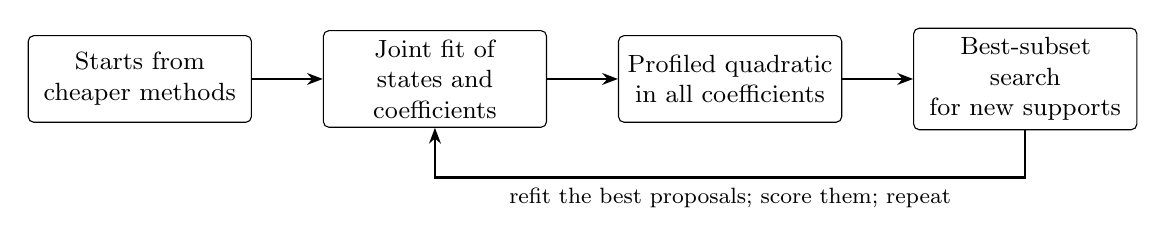
\begin{tikzpicture}[
  box/.style={draw, rounded corners=2pt, align=center, minimum height=11mm, text width=26mm, font=\small},
  arr/.style={-{Stealth[length=2mm]}, thick},
  node distance=9mm]
\node[box] (start) {Starts from\\cheaper methods};
\node[box, right=of start] (fit) {Joint fit of\\states and coefficients};
\node[box, right=of fit] (quad) {Profiled quadratic\\in all coefficients};
\node[box, right=of quad] (subset) {Best-subset search\\for new supports};
\draw[arr] (start) -- (fit);
\draw[arr] (fit) -- (quad);
\draw[arr] (quad) -- (subset);
\draw[arr] (subset.south) -- ++(0,-6mm) -| node[pos=0.25, below, font=\footnotesize] {refit the best proposals; score them; repeat} (fit.south);
\end{tikzpicture}
\caption{Structure of the method. The joint fit is the expensive step and the best-subset search is cheap, so most candidate models are evaluated only on the quadratic.}
\label{fig:overview}
\end{figure}

\begin{algorithm}[t]
\caption{PJSS (white-noise path). Defaults: $\rho=0.03$, $c=2$, $k_{\max}=5$, two candidates per size, ten finalists, two rounds.}
\label{alg:pjss}
\begin{algorithmic}[1]
\Require samples $y_{0:n-1}$, step $\Delta t$, library $\theta$
\State scale coordinates by RMS; $\hat\sigma\gets$ high-frequency floor; $s\gets$ spectral sub-step rule
\State $\Tset,\Vset\gets$ train / every-third-sample hold-out; initial states by Savitzky--Golay smoothing
\State $\mathcal P\gets$ \Call{FitJoint}{$\Sset_0$} for each start support $\Sset_0$ (weak $\chi^2_s$, hybrid, flow)\Comment{banded LM, \cref{sec:objective}}
\State $\hat a\gets$ lag-1 autocorrelation of best start's residuals; \textbf{if} $\mathrm{mean}(\hat a)>0.6$ \textbf{then} use the AR(1) likelihood
\State recalibrate $\hat\sigma\gets\max(\hat\sigma,1.4826\,\MAD(r))$ if larger by $>10\%$ (refit starts); $\varphi\gets$ autocorrelation inflation
\State $F^\star\gets\argmin_{F\in\mathcal P}\mathrm{Score}(F)$\Comment{\cref{eq:score}, prior \cref{eq:prior}}
\For{round $=1,2$}
  \State $(A,b)\gets$ profiled quadratic at $F^\star$ over all $MD$ coefficients\Comment{\cref{eq:profile}}
  \For{$j=1,\dots,D$}
    \State project the other equations' active columns out of $(A,b)$
    \State $\mathcal C_j\gets$ top-2 subsets per size $k\le k_{\max}$ (exhaustive; beam if $>2.5\times10^5$)
  \EndFor
  \State proposals $\gets$ single-equation replacements $\cup$ $\prod_j\text{top-2}_Q(\mathcal C_j)$; rank unfitted ones by $Q$
  \State $\mathcal P\gets\mathcal P\,\cup$ \Call{FitJoint}{} on the 10 best, warm-started at $F^\star$'s states
  \State $F\gets\argmin_{\mathcal P}\mathrm{Score}$; \textbf{if} $F=F^\star$ \textbf{break}; $F^\star\gets F$
\EndFor
\State refit $F^\star$ on all samples, then at $\rho=0.001$ (fixed support; states and coefficients updated)
\State \Return coefficients, ambiguity flag (gap $<2\lambda$), per-term BIC weights over $\mathcal P$
\end{algorithmic}
\end{algorithm}

\subsection{Joint objective for a fixed support}
\label{sec:objective}
The latent states $u_k\in\R^D$ live on a sub-grid with $s$ steps per sample, $k=0,\dots,(n-1)s$, with step $h=\Delta t/s$. Sample $i$ sits at grid index $o(i)=is$. Every third sample ($i\equiv 2 \bmod 3$) is held out of the data term. This gives training samples $\Tset$ and validation samples $\Vset$. For a support $\Sset$ we minimise over $(\bu, C)$ with $C_{mj}=0$ for $(m,j)\notin\Sset$:
\begin{equation}
\begin{split}
J(\bu,C) \;=\;& \sum_{i\in\Tset}\sum_{j=1}^{D} \rho_c\!\left(\frac{u_{o(i),j}-y_{ij}}{\sigma_j}\right)\\
&+\; \sum_{k}\sum_{j=1}^{D}\left(\frac{u_{k+1,j}-u_{k,j}-h\,\theta(m_k)^\top C_{:,j}}{\rho\,\sigma_j}\right)^{2},
\qquad m_k=\tfrac12(u_k+u_{k+1}).
\end{split}
\label{eq:objective}
\end{equation}
The first term pulls the states toward the measurements, and the second pulls them toward a solution of the candidate model, so a support that cannot explain the data leaves a residual in one term or the other. In the first term, $\rho_c(r)=r^2$ for $|r|\le c$ and $2c|r|-c^2$ otherwise, which is twice the Huber loss~\citep{huber1964robust}, with $c=2$. The second term is a soft midpoint-rule dynamics constraint with relative weight $\rho=0.03$. The noise scale $\sigma_j$ is calibrated (\cref{sec:calibration}).

\paragraph{Banded Levenberg--Marquardt solve.}
We minimise \eqref{eq:objective} by Levenberg--Marquardt~\citep{levenberg1944,marquardt1963} with iteratively reweighted Huber weights. The states are interleaved in time, so each dynamics residual couples only $u_k$ and $u_{k+1}$. The Gauss--Newton matrix therefore has the block form
\begin{equation}
\begin{pmatrix} A_{uu} & A_{uc}\\ A_{uc}^\top & A_{cc}\end{pmatrix}
\begin{pmatrix}\delta\bu\\ \delta\bc\end{pmatrix} = -\begin{pmatrix} g_u\\ g_c\end{pmatrix},
\label{eq:normal}
\end{equation}
where $A_{uu}$ is symmetric banded with upper bandwidth $2D-1$, and $A_{uc}$, $A_{cc}$ form a dense border in the $|\Sset|$ active coefficients. We solve \eqref{eq:normal} by one banded Cholesky factorisation with $|\Sset|+1$ right-hand sides and the Schur complement $A_{cc}-A_{uc}^\top A_{uu}^{-1}A_{uc}$. Each iteration is linear in the number of latent states. The initial states are the samples, smoothed by a Savitzky--Golay filter and interpolated onto the sub-grid.

\subsection{Profiled quadratic and subset proposals}
\label{sec:proposals}
Let $(\bu^\star, C^\star)$ be the current best fit. We form \eqref{eq:normal} at that point for \emph{all} $MD$ coefficients, including inactive ones, and eliminate the states:
\begin{equation}
H = A_{cc}-A_{uc}^\top A_{uu}^{-1}A_{uc},\qquad g = g_c - A_{uc}^\top A_{uu}^{-1}g_u,\qquad
\bc^\dagger = \bc^\star - H^{-1}g .
\label{eq:profile}
\end{equation}
With $H=LL^\top$, set $A=L^\top$ and $b=L^\top\bc^\dagger$. Then
\begin{equation}
q(\bc) = \lVert A\bc-b\rVert^2
\end{equation}
is, up to a constant, the quadratic obtained by eliminating state increments from the local Gauss--Newton model. This is the \emph{profiled quadratic}. The displayed inverse and Cholesky factorisation assume positive definiteness. In the implementation we symmetrise $H$ and add $10^{-10}\operatorname{tr}(H)/(MD)$ to its diagonal before solving, so the computed proposal uses a regularised quadratic. A single banded solve with $MD+1$ right-hand sides gives $H$; scoring a support then requires only a small least-squares solve.

\paragraph{Why profile the states?} A coefficient change can be partly accommodated by changing the estimated trajectory. Fixed-state proposals use $A_{cc}$ and $g_c$ and ignore this adjustment; the Schur terms in \eqref{eq:profile} account for it within the local quadratic. Profiling therefore changes the geometry used to rank supports before any nonlinear refit. It does not solve the nonlinear state-estimation problem for every candidate. Its value is tested separately from subset enumeration in \cref{sec:ablation}, and all retained proposals are checked by joint refitting.

\paragraph{Proposals.} Searching all equations at once would multiply the number of subsets across equations, so proposals are generated per equation. For equation $j$, the columns of the \emph{other} equations' currently active coefficients are projected out of $A$ and $b$ (orthogonal complement of their span, via SVD). We then run exhaustive best-subset regression over the $M$ columns of equation $j$: for every size $k=1,\dots,k_{\max}$ ($k_{\max}=5$) we keep the two subsets with the smallest residual sum of squares, computed with normalised columns and a $10^{-10}$ ridge. The empty per-equation support is also included. For $M=20$ the nonempty search enumerates $\sum_{k=1}^{5}\binom{20}{k}=21{,}699$ subsets per equation. When the count would exceed 250{,}000 (degree 4 and 5 libraries), a beam search of width 60 over the same normalised Gram system replaces enumeration. Two kinds of joint proposal are formed:
\begin{enumerate}[leftmargin=*,itemsep=1pt]
\item \emph{single-equation replacements}: the current support with equation $j$'s terms replaced by each candidate;
\item \emph{combinations}: each equation's candidates are ranked by the quadratic BIC $Q(\Sset')=\min_{\bc}\lVert A_{\Sset'}\bc-b\rVert^2+|\Sset'|\log(Dn)$ (other equations at their current supports), and the Cartesian product of the top two per equation is added ($2^D$ combinations, capped at 1{,}024 for $D>3$).
\end{enumerate}
All proposals not yet fitted are ranked by $Q$. The top ten are refitted with the full nonlinear objective \eqref{eq:objective}, starting from the current states and the quadratic's coefficients. The best-scoring fit becomes the new expansion point, and the procedure repeats for at most two rounds, stopping early if the best fit does not change. Enumeration is exhaustive only within each per-equation size limit; the combined support search and nonlinear fits are not globally certified.

\subsection{Score and complexity prior}
\label{sec:score}
A fitted candidate $\Sset$ with states $\bu$ is scored by
\begin{equation}
\mathrm{Score}(\Sset) \;=\; \underbrace{\sum_{i\in\Tset}\sum_j\rho_c(r_{ij})}_{\text{train misfit}} + \underbrace{\sum_k\sum_j(\cdot)^2}_{\text{dynamics}} + \underbrace{\sum_{i\in\Vset}\sum_j\rho_c(r_{ij})}_{\text{held-out misfit}} + \varphi\,\kappa(\Sset)\,\log(Dn),
\qquad r_{ij}=\frac{u_{o(i),j}-y_{ij}}{\sigma_j}.
\label{eq:score}
\end{equation}
The masked samples are excluded from each joint fit's observation-data term. They still inform the starts, scaling, spectral grid, noise calibration and AR(1) routing, so this is a masked-fit selection criterion, not independent out-of-sample validation. This is a practical criterion, not an approximation to a marginal likelihood. Its penalty is inspired by BIC~\citep{schwarz1978bic}, with two modifications:
\begin{itemize}[leftmargin=*,itemsep=1pt]
\item \textbf{Autocorrelation inflation} $\varphi\ge 1$ (\cref{sec:calibration}). It compensates for correlated residuals, which make the effective number of independent observations smaller than $Dn$.
\item \textbf{Degree-weighted prior.} Instead of counting terms, we use $\kappa(\Sset)=\sum_{(m,j)\in\Sset}w(\deg\theta_m)$ with
\begin{equation}
w(d)=\max\bigl(0.1,\;1+0.2\,(d-1.5)\bigr),
\label{eq:prior}
\end{equation}
so a constant costs $0.7$, a linear term $0.9$, a quadratic $1.1$ and a cubic $1.3$ times $\log(Dn)$. The penalty stays close to BIC's level for typical low-degree models, but low-degree terms are preferred, as in the complexity measures of symbolic regression~\citep{schmidt2009distilling,cranmer2023pysr}. Sine and cosine terms get weight 1. The strength 0.2 was chosen from three values on development data.
\end{itemize}
The prior enters only the score of fitted candidates; the proposal ranking $Q$ uses the plain term count. After selection, the chosen support is refitted with all samples in the data term, then once more with a stiffer dynamics weight $\rho=0.001$. This last refit removes coefficient shrinkage and does not change the support.

\subsection{Self-calibration}
\label{sec:calibration}
PJSS selects sparsity without a user-specified threshold. It still has fixed internal constants, including the dynamics weight, maximum subset size and proposal budget. These were chosen on development data; \cref{tab:sensitivity} reports their sensitivity.
\paragraph{Noise scale and penalty inflation.}
The noise scale starts from a high-frequency estimate based on fourth-order differences, which sees white noise but misses slowly correlated noise. After the starts are fitted, it is raised to the robust scale of the sample residuals if that scale is more than 10\% larger, and the starts are refitted. Correlated residuals also carry less information than their number suggests, so the BIC penalty is multiplied by $\varphi\ge1$, an estimate of the integrated autocorrelation of the residuals (\cref{app:impl}).

\paragraph{Correlated noise.}
For strongly correlated errors we replace the data term with the exact Gaussian likelihood of AR(1) errors per component, $e_{i,j}=a_j e_{i-1,j}+\nu_{i,j}$. Whitening these errors couples only neighbouring observations, so the system stays banded and a fit stays linear in the record length. Spurious terms that bend the latent trajectory toward slow noise can still win under this likelihood, so the penalty in \eqref{eq:score} becomes $\lambda(a)\,\varphi\,\kappa(\Sset)\log(Dn)$, with a heuristic factor $\lambda(a)$ and with $\varphi$ computed from the whitened residuals. The AR(1) model is used if and only if the mean of $\hat a$, estimated from the residuals of the best start, exceeds $0.6$.

\paragraph{Discretisation.} Two further quantities are set from the data (\cref{app:impl}). The number of sub-steps per sample, between 2 and 12, follows the spectrum of the data, and a floor on the noise scale keeps the midpoint rule's truncation error from being fitted as if it were signal on noise-free data.

\subsection{Starts and outputs}
\label{sec:starts}
\label{sec:flag}
The search is seeded with truth-free answers from cheaper methods, chiefly the \emph{weak $\chi^2_s$ selector}, an exhaustive best-subset weak SINDy~\citep{messenger2021wsindy} with a self-calibrated size rule. A score gap below 2 (or $2\lambda$ on the AR(1) path) flags ambiguity within the fitted candidate pool. This threshold is motivated by the evidence scale of \citet{kass1995bayes}, but our heuristic score does not yield a Bayes factor. Exponentiated score weights give per-term inclusion diagnostics, with development-fitted calibration for the default library (\cref{app:impl}). Neither output detects missing library terms reliably.

\section{Experimental protocol}
\label{sec:protocol}

\subsection{Systems, data and metrics}
\paragraph{Core benchmark.} Ten polynomial chaotic systems of degree $\le3$ in $D=3$: Lorenz~\citep{lorenz1963}, R\"ossler~\citep{rossler1976}, Chen~\citep{chen1999}, Halvorsen, Sprott A--E and Rabinovich--Fabrikant~\citep{rabinovich1979}. Each run starts at a random point on the attractor and has $N\in\{500,2000\}$ samples, with 10 seeds per cell. Noise is added at $\eta\in\{1,5,10,20\}\%$ of each coordinate's standard deviation, so one archive has 800 runs. The variants are AR(1) coloured noise ($a=0.8$), Student-$t_3$ noise and four-times coarser sampling.

\paragraph{Held-out systems.} This set adds eleven further polynomial chaotic systems (880 runs per archive).

\paragraph{External benchmark.} The \texttt{dysts} database (v0.96)~\citep{gilpin2021dysts} has 135 continuous-time chaotic systems, of which 77 lie in our libraries: 61 three-dimensional systems of degree $\le3$, and 16 systems of dimension 4--6 and degree $\le 2$. Forty-nine of the 77 are new to us; the other 28 overlap with our systems or share a support with one of them. The test archive has 6{,}160 runs and was generated before any method was run on it.

\paragraph{Metrics.} The primary metric is \emph{exact support recovery}: the estimated nonzero pattern equals the true one in every equation. We also report term-level F1 and relative coefficient error $\lVert\hat C-C\rVert_F/\lVert C\rVert_F$. Truth is used for scoring, explicitly labelled oracle references and diagnostics, not by PJSS at inference. Comparisons are paired by run; ``W/L'' counts recoveries unique to each method. We report central confidence intervals in the main text and detailed paired tests in the appendix. Runs nest within systems, so system-resampled intervals are used where available to assess transfer across systems; run-level tests describe the sampled runs.

\subsection{Development and test separation}
\label{sec:freezing}
``Pre-registered'' below denotes a prospective protocol recorded in the repository before its experiment, not an independently registered study.
Defaults were chosen on development archives. Each test archive uses new seeds, and each test pass ran a checksummed model with no setting changed during the pass. Test results did inform later work: the Gaussian loss of \cref{sec:noise} and the noise floor each followed a test finding, and each was redeveloped on development data and confirmed on a fresh pre-registered archive. Test archives other than \texttt{dysts} were also evaluated more than once (\cref{sec:limitations}). The test archives are the \emph{sealed} and \emph{confirmation} white-noise archives, held-out systems, the coloured, $t_3$ and coarse variants, the large-library and $D>3$ archives, and \texttt{dysts}. The \emph{hard 40} are the Lorenz, Chen, R\"ossler and Rabinovich--Fabrikant runs of the confirmation archive at 20\% noise and $N=2000$. They were chosen \emph{because} they are hard for our methods, so they serve only as a stress test. The head-to-head, cost study and sensitivity sweep use the final method; the other test tables predate small refinements that change the \texttt{dysts} rate by 0.001 (\cref{app:tables}).

\subsection{Baselines}
\label{sec:baseline-config}
We compare with the SINDy variants in pysindy~\citep{desilva2020pysindy,kaptanoglu2022pysindy}, including E-SINDy and MIOSR; with WSINDy~\citep{messenger2021wsindy} and ARGOS~\citep{egan2024argos}; with the symbolic regressors PySR~\citep{cranmer2023pysr} and ODEFormer~\citep{dascoli2024odeformer}; and with the joint-state methods DEDi~\citep{meissner2024dedi}, using the authors' code and full grid, and ODR-BINDy~\citep{fung2025odrbindy}, using our Python port. Threshold-based methods get two truth-free rules, 5-fold regression-row cross-validation (CV) and AICc~\citep{mangan2017model}, and two that use the truth: one threshold \emph{tuned} per evaluation set, and the per-run \emph{oracle}. Costly baselines ran on subsamples of \texttt{dysts}. Configurations are in \cref{app:baselines}.


CV partitions precomputed regression rows. SFD rows follow time order but use full-record preprocessing; weak rows are randomly located, potentially overlapping temporal domains. Neither is a fully isolated temporal holdout. Historical weak-feature baselines also constructed random domains before setting the run seed. We preserve those recorded results, disclose this reproducibility limitation, and distinguish the corrected implementation and targeted check in \cref{app:baseline-audit}.

\paragraph{Method versions.} \Cref{sec:method} describes v1.2. The frozen v1.0 tables retain their original results; v1.0.1 fixes empty-support handling, v1.1 changes AR(1) residual loss to Gaussian, and v1.2 adds the discretisation floor. The DEDi comparisons and timing study use v1.2. \Cref{app:tables} maps versions to results; values from different versions are not pooled as one experiment.

\section{Results}
\label{sec:results}

\subsection{Recovery on the test archives}
\label{sec:main}
\label{sec:dysts}

\begin{table}[t]
\centering
\caption{Exact support recovery on the test archives. \emph{Weak}: the weak best-subset selector. \emph{Base}: our method without the prior or AR(1) model. The first six rows use our 3-D archives, and the \texttt{dysts} archive was generated before any method was run on it. The PJSS column reports frozen v1.0 before later refinements, which raise the coloured row to 0.812, and 0.805 on a fresh archive (\cref{sec:noise}). Paired tests are in \cref{tab:main,tab:dysts}.}
\label{tab:summary}
\small
\begin{tabular}{@{}lrccc@{}}
\toprule
Archive & Runs & Weak & Base & \textbf{PJSS v1.0} \\
\midrule
Sealed (white) & 800 & 0.752 & 0.881 & \textbf{0.889} \\
Confirmation (white) & 800 & 0.754 & 0.868 & \textbf{0.886} \\
Held-out systems & 880 & 0.907 & 0.933 & \textbf{0.941} \\
Coloured AR(1), $a=0.8$ & 800 & 0.645 & 0.674 & \textbf{0.761} \\
Heavy-tailed $t_3$ & 800 & 0.755 & 0.889 & \textbf{0.905} \\
Coarse sampling $\times4$ & 800 & 0.654 & \textbf{0.790} & 0.784 \\
\midrule
\texttt{dysts}, all 77 systems & 6{,}160 & 0.675 & 0.879 & \textbf{0.890} \\
\texttt{dysts}, 49 new systems & 3{,}920 & 0.591 & 0.840 & \textbf{0.853} \\
\bottomrule
\end{tabular}
\end{table}

\Cref{tab:summary} gives the main result. The joint method outperforms the weak selector on every archive, and the gains are largest at high noise. On a fresh pre-registered archive of 120 runs of Lorenz, Chen and R\"ossler at 20\% noise and $N=2000$, it recovers 112, against 0 for the weak selector. Coarse sampling is the one archive where it falls below the base model (4 paired wins, 9 losses).

Accuracy carries over to the external benchmark, which we did not design: 0.890 overall and 0.853 on the 49 new systems. Runs of one system are not independent, so we also resampled systems, which gives 95\% intervals of $[0.841,0.931]$ and $[0.783,0.914]$. Of the 77 systems, 56 score at least 0.9 and five score below 0.5. Those five share one failure, a true term that is tiny relative to the others or that acts on a fast, stiff time scale. Results for dimensions up to 10, larger libraries and the non-chaotic ODEBench collection are in \cref{app:more}.

\subsection{Separating subset search from profiling}
\label{sec:ablation}
We use leave-one-out ablations and a cumulative ladder on 576 runs: sealed white noise (160), coloured noise (89), the hard 40, and three-dimensional \texttt{dysts} (287). No settings were tuned on these subsets. \Cref{fig:ladder} shows the ladder; full rates and paired tests are in \cref{tab:ablation,app:ablation-detail}.
\begin{figure}[t]
\centering
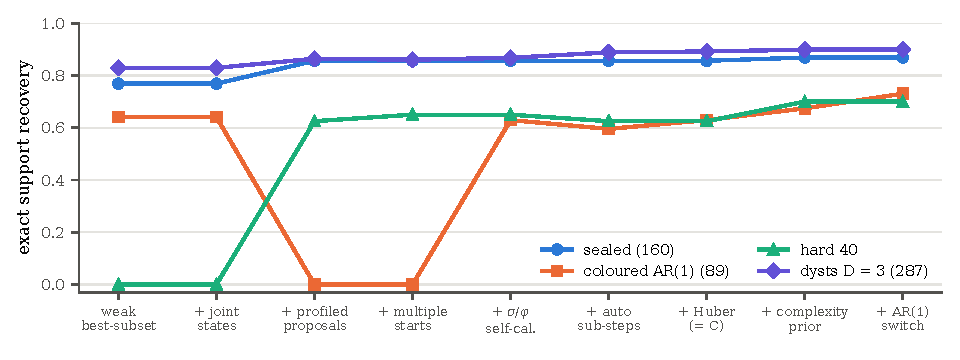
\includegraphics[width=0.92\linewidth]{figures/ablation_ladder.pdf}
\caption{Cumulative ladder from the weak best-subset selector to our method. Up to the last rung the white-noise likelihood is used. Refitting the weak answer jointly (second rung) cannot change its support. The profiled-quadratic proposals give the largest step on white noise, and without self-calibration they overfit every coloured run.}
\label{fig:ladder}
\end{figure}

\paragraph{Subset proposals.} Removing proposals loses 32 exact recoveries and gains none; replacing exhaustive selection with forward stepwise search loses 28 and gains none. On the hard 40, joint refitting of the weak start alone recovers no runs, all starts refitted without proposals recover 19, proposals from the weak start recover 27, and the full method recovers 28. Searching combinations of terms is therefore the principal source of the improvement over refitting existing supports.

\paragraph{Profiling.} A separate prospective ablation builds proposals from $A_{cc}$ and $g_c$, holding the states fixed instead of eliminating their increments. PJSS recovers 490/576 runs versus 480/576 for this variant, with 15 paired wins and 5 losses. On the hard 40 it recovers 28 versus 24; on coloured noise the fixed-state variant has one more recovery. Profiling therefore adds a smaller, setting-dependent gain: it changes how candidates are ranked by accounting for local state adjustment, while both variants retain exhaustive subset proposals and nonlinear joint refits.

\paragraph{Calibration.} Under a white-noise likelihood, proposals overfit every coloured run without noise-scale and penalty calibration; calibration restores recovery in the ladder. Its effect on white noise is negligible. Gaussian loss improves the AR(1) path, motivating the separately confirmed update in \cref{sec:noise}. Other ablations and coefficient errors are reported in \cref{app:ablation-detail}.


\subsection{Comparison with standard baselines}
\label{sec:baselines}

\begin{figure}[t]
\centering
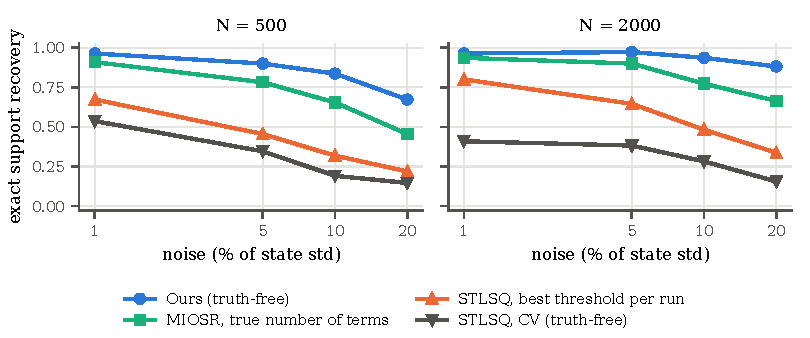
\includegraphics[width=0.82\linewidth]{figures/baselines_noise.pdf}
\caption{Exact recovery on the 880 paired \texttt{dysts} runs, by noise level and record length. Two of the four curves use the truth: STLSQ with the best threshold chosen per run, and MIOSR given the true number of terms in each equation. Each point is the mean of 110 runs.}
\label{fig:baselines-noise}
\end{figure}

PJSS has higher exact recovery than each tested standard baseline on the paired subsets, including the oracle references (\cref{fig:baselines-noise}; all baselines are in \cref{tab:baselines}). The strongest truth-free competitors are SINDy with STLSQ (0.306 against 0.891) and PySR (0.444 against 0.929). The best reference that uses the truth is MIOSR given the true number of terms (0.759), which our truth-free method still beats 123/7. The per-run oracle of the threshold-based baselines is 1.4--2.4 times their best truth-free rule, which confirms that the threshold choice limits them, although it does not explain the whole gap. PySR and ODEFormer are general-purpose methods, and exact recovery is a harsh metric for them. On the hard 40, our method recovers 28 and our Python port of ODR-BINDy, given the true noise level, 14 in its better setting at about 2\,h per run. This comparison concerns the port; equivalence with the original solver has not been validated.

\subsection{Comparison with DEDi}
\label{sec:h2h}
\label{sec:hard}
The closest competitor is the joint-state method DEDi. We pre-registered a comparison on 80 runs, 16 per condition, drawn at random from five archives of the 10 core systems (\cref{tab:dedi}). It therefore covers systems used in development; a second comparison on new systems follows. The hard condition covers Lorenz, Chen and R\"ossler, without Rabinovich--Fabrikant. The primary test is exact recovery against DEDi's default selection by validation error. Secondary analyses are DEDi selecting by BIC, and an oracle that counts a run as exact if any of DEDi's 35 fits is exact, which recovers 64.

\begin{table}[t]
\centering
\caption{Pre-registered comparison with DEDi on 80 random runs: number of runs recovered exactly. \emph{Val} is DEDi's default selection by validation error and \emph{BIC} its alternative. Paired tests are in \cref{tab:h2h}.}
\label{tab:dedi}
\small
\begin{tabular}{@{}lcccc@{}}
\toprule
Condition & $n$ & \textbf{Ours} & DEDi val & DEDi BIC \\
\midrule
Hard (20\%, $N=2000$) & 16 & 15 & 13 & 15 \\
White (10--20\%) & 16 & 14 & 14 & 14 \\
Coloured AR(1) (10--20\%) & 16 & 10 & 5 & 5 \\
Heavy-tailed $t_3$ (10--20\%) & 16 & 14 & 12 & 13 \\
Short ($N=500$, 5--10\%) & 16 & 13 & 11 & 14 \\
\midrule
\textbf{All} & 80 & \textbf{66} & 55 & 61 \\
\bottomrule
\end{tabular}
\end{table}

PJSS recovers 66/80 runs, compared with 55/80 for DEDi's default validation selection and 61/80 for BIC selection. The paired difference for BIC, DEDi minus PJSS, is $-0.062$ (95\% CI $[-0.140,+0.011]$): it meets the pre-specified noninferiority margin of 0.10 but does not establish superiority. Without coloured noise, the two recover the same 56/64 runs. Detailed paired tests and the device sensitivity analysis are in \cref{app:paired}.

A second prospective comparison uses 64 runs of 35 three-dimensional \texttt{dysts} systems outside our development benchmarks. PJSS recovers 53, against 36 with DEDi's validation selection, 41 with BIC and 44 under its oracle (\cref{tab:h2h-dysts}). Resampling systems gives 95\% intervals for the differences of $[-0.413,-0.119]$ and $[-0.344,-0.044]$, respectively; this clustering check was post hoc, with the reproducible resampling procedure in \cref{app:bootstrap}. The advantage is concentrated at 1--5\% noise (29/32 versus 14/32 and 19/32); at 10--20\% noise, PJSS recovers 24/32 versus 22/32 for either selection. These comparisons have different designs and neither covers $D>3$.

\begin{table}[t]
\centering
\caption{Pre-registered comparison of PJSS v1.2 with DEDi on 64 runs of the 35 three-dimensional \texttt{dysts} systems new to us (8 runs per combination of noise and $N$). W/L: runs only ours / only DEDi gets exactly right. The difference is the DEDi exact rate minus ours, with Newcombe's paired 95\% CI. The oracle uses the truth.}
\label{tab:h2h-dysts}
\small
\begin{tabular}{@{}lcccc@{}}
\toprule
Noise & $n$ & \textbf{Ours} & DEDi val & DEDi BIC \\
\midrule
1\% & 16 & 15 & 5 & 8 \\
5\% & 16 & 14 & 9 & 11 \\
10\% & 16 & 14 & 13 & 13 \\
20\% & 16 & 10 & 9 & 9 \\
\midrule
\textbf{All} & 64 & \textbf{53} & 36 & 41 \\
W/L ($p$) & & & 19/2 (0.0002) & 15/3 (0.008) \\
Difference & & & $-0.266$ & $-0.188$ \\
95\% CI & & & $[-0.384,-0.137]$ & $[-0.306,-0.064]$ \\
\midrule
DEDi oracle (uses truth) & 64 & 53 & \multicolumn{2}{c}{44, 12/3 (0.04)} \\
\bottomrule
\end{tabular}
\end{table}

\subsection{Computational cost}
\label{sec:cost}

\begin{figure}[t]
\centering
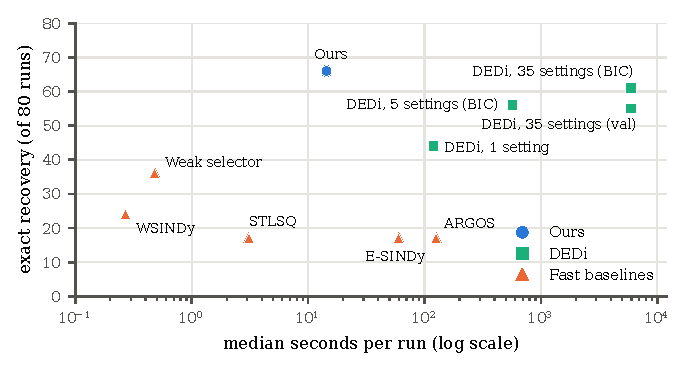
\includegraphics[width=0.66\linewidth]{figures/accuracy_cost.pdf}
\caption{Accuracy against cost on the 80 head-to-head runs. Every method picks its sparsity without the truth. Times are median wall seconds per run on a fully loaded machine. Ours and the fast baselines ran on one CPU core; DEDi ran on a GPU shared by 10 processes for 73 of the 80 runs. Exact values are in \cref{tab:fast}.}
\label{fig:cost}
\end{figure}

\Cref{fig:cost} reports accuracy and wall-clock cost on a loaded NVIDIA GB10 machine; these timings compare execution setups rather than intrinsic costs. A separate measurement on three cases gives about 5\,s per PJSS run. DEDi uses 4{,}374--34{,}006 aggregate single-thread task-seconds across three concurrent CPU workers, or 501--4{,}462\,s with one GPU process. The CPU totals sum elapsed times for 35 grid pairs; they are not measured serial full-grid wall times. Sharing pairs across workers deviated from the prospective CPU protocol; the GPU measurement ran as planned. Two runs are Sprott~A and one is Rabinovich--Fabrikant, which neither method recovers, so these ratios should not be generalised to all systems (\cref{app:timing-detail}).

The computational difference comes from support search. PJSS performs about 21 joint fits and screens candidate subsets cheaply; DEDi performs a backward-elimination sequence for each grid setting. Smaller DEDi budgets reduce cost but also recovery: one setting recovers 44/80 runs, and five settings with BIC recover 56/80. WSINDy is about 50 times faster than PJSS on the loaded-machine comparison and recovers 24/80. Scaling results are in \cref{app:more}.

\subsection{Coloured noise}
\label{sec:noise}
Coloured AR(1) noise is the hardest setting, because slow noise excursions resemble dynamics. The base model gains only 3 points over the weak selector (0.674 against 0.645), and the AR(1) likelihood with the automatic switch raises this to 0.761. The switch fired on 100\% of coloured test runs and on 0\% of sealed and confirmation runs. The ablation then showed that Huber loss hurts inside the AR(1) likelihood (\cref{sec:ablation}). That finding came from a test subsample, so we redeveloped the change on development data and pre-registered a fresh coloured archive of 800 runs, on which the Gaussian loss raises exact recovery from 0.754 to 0.805 (43 paired wins, 2 losses). It changed 0 of 1{,}600 answers on the white and $t_3$ archives.

\subsection{Real data}
\label{sec:realdata}
Our real-data tests are negative or anecdotal.

\paragraph{Lynx and hare.} On the 21 annual Hudson's Bay pelt counts, a standard example that E-SINDy~\citep{fasel2022esindy} solves, the model returns a degenerate answer whose integration diverges, and it does not flag it. These data are far below the $N=500$--2{,}000 regime the method was built for. On a cubic-spline resampling (201 points) it finds all four Lotka--Volterra terms plus one weak extra term, but the method was never validated on interpolated data, so this is an anecdote.
% Source: docs/reports/real_data.md; results_real/lynx_hare.json, results_real/lynx_hare_v101.json.

\paragraph{Measured pendulums.} We found no public recording of a chaotic system whose accepted model is polynomial, so we used the multi-arm pendulum rig of \citet{kaheman2023pendulum} with a pre-registered protocol. For the single pendulum, the coordinates $(\sin\theta,\cos\theta,\dot\theta)$ put the accepted model $\ddot\theta=A\sin\theta-B\dot\theta$ in the library. The method fails the pre-specified support criterion. It finds the gravity term ($A$ within 0.2\%) and both kinematic terms, but it drops the damping term and adds 11 small terms, which stand in for dissipation. No pysindy baseline has the exact support anywhere on its threshold path. However, $\sin^2\theta+\cos^2\theta=1$ and its multiples make the cubic library dependent on this embedding manifold. Distinct supports can represent the same dynamics there, so failure to recover the selected support alone does not establish dynamical failure; an equivalence-aware evaluation was not performed.

The double pendulum's accepted model is rational in $\cos(\theta_1-\theta_2)$, so it lies outside every library we have, and our method is worse than the pysindy baselines: its forecast stays valid for 0.024--0.127\,s, against 0.47--1.47\,s for SINDy and about 0.13\,s for persistence. It never recovers the identities $\dot\theta_i=\omega_i$, which the equation-wise baselines find almost exactly, and it does not flag the answer. Our hypothesis, not tested further, is that when some equations cannot be represented, the joint objective distorts the ones that can, whereas equation-wise regression keeps a misspecified equation from contaminating the others.
% Source: docs/reports/real_data2.md; results_real2/{single,double}_*.json, results_real2/tables.md.
% Pre-registration: results_real2/PREREGISTRATION.md; data sources and sha256: results_real2/SOURCES.md.

\section{Limitations}
\label{sec:limitations}

PJSS is evaluated primarily on uniformly sampled, fully observed trajectories whose true equations lie in the library. The positive results do not establish robustness to process noise, irregular sampling, inputs or library misspecification. The measured-pendulum tests fail, and the ambiguity flag can remain silent on inaccurate models (\cref{sec:realdata}). The confidence weights are calibrated diagnostics for the evaluated setting, not guarantees of correctness.

The search is local in its quadratic approximation and restricted in its supports: exhaustive proposals use at most five terms per equation, larger libraries use approximate beam search, and only two proposal rounds are used by default. Fixed constants were selected during development; the one-at-a-time sensitivity sweep does not test their interactions. The degree prior favours the low-degree systems in the benchmarks. Coloured-noise handling is implemented only for $D=3$, and higher-dimensional tests use degree-2 libraries. The partial-observation extension recovers 146/240 runs on three systems but only 7/60 with two latent components (\cref{app:partial}).

Several test archives were reused during development, and runs within a system are dependent. We distinguish fresh confirmations and system-resampled intervals from run-level analyses. Comparisons using an unvalidated ODR-BINDy port, reduced-budget DAHSI-style baseline, or published ODEBench figure values have narrower interpretations than the official-code paired comparisons. The three timing cases do not establish a universal speedup. Full qualifications are retained in \cref{app:limitations-detail}.

\section{Conclusion}
\label{sec:conclusion}

PJSS combines joint state--coefficient estimation with profiled quadratic subset proposals. Profiling accounts for local trajectory adjustment, subset search explores competing term combinations, and nonlinear refits check the proposed supports. The ablations attribute most of the recovery gain to subset proposals, with a smaller additional gain from profiling. Fixed defaults and data calibration remove the need for a user-specified sparsity threshold on the evaluated benchmarks.

On simulated in-library systems, PJSS improves recovery over the tested sparse-regression baselines and reduces the cost of comparison with full-grid DEDi. The two methods tie on some conditions, while PJSS recovers more runs in the new-system comparison. Real-data and misspecification tests remain negative, so detecting model inadequacy is a priority before broader scientific use.

\paragraph{Reproducibility.} The accompanying code contains benchmark runners, stored results, checksum manifests and executable audits. \path{docs/paper/scripts/verify_numbers.py} recomputes headline summaries; figure generation also reads saved results. The main full-observation archives are available and match their hashes. Four secondary-study originals are missing locally, and regeneration did not reproduce their hashes (\cref{app:data-audit}); those historical results cannot currently be reproduced exactly. A public artifact location and the original benchmark environment remain release requirements. The README documents commands, versions and evidence limitations.

\section*{Declarations}\paragraph{AI use.} Generative AI tools were used in research and experiment design, code development, and manuscript drafting and revision. The author assumes responsibility for all content.


\bibliographystyle{plainnat}
\bibliography{refs}

\appendix
\section{Implementation details}
\label{app:impl}

\paragraph{Solver.} The Levenberg--Marquardt damping is Marquardt's, $\mu(1+\diag)$. A step is accepted if the cost decreases ($\mu\leftarrow\mu/3$) and rejected otherwise ($\mu\leftarrow 4\mu$). We stop after at most 40 iterations or at a relative decrease below $10^{-7}$. The initial states are the samples with held-out values linearly interpolated, smoothed by a Savitzky--Golay filter (window 21, order 3) and interpolated onto the sub-grid.

\paragraph{Noise scale and penalty inflation.} The initial $\hat\sigma_j$ is $\MAD(\Delta^4 y_j)/(0.6745\sqrt{70})$. After the starts are fitted, let $r_i=y_i-u_{o(i)}$ be the sample residuals of the best start, and $\sigma^{r}_j = 1.4826\,\MAD(r_{\cdot j})$. If any $\sigma^r_j>1.1\,\hat\sigma_j$, we set $\hat\sigma\leftarrow\max(\hat\sigma,\sigma^r)$ componentwise and refit the starts. The inflation is $\varphi=\max\bigl(1, \tfrac1D\sum_j[1+2\sum_{\ell\ge1}\hat\rho_{j,\ell}]\bigr)$, where $\hat\rho_{j,\ell}$ is the lag-$\ell$ autocorrelation of $r_{\cdot j}/\sigma^r_j$. The sum is truncated at the first lag with $\hat\rho<0.05$, and at most 50 lags.

\paragraph{Discretisation floor.} On noise-free data the estimated $\hat\sigma$ collapses, and the midpoint rule's own truncation error becomes the largest ``noise'' left. The dynamics term then rewards small smooth extra terms that absorb this deterministic error, so the floor limits the discretisation error to at most one term's penalty in the score. The local truncation error $\tau_k$ of the midpoint step is computed along the best start's states with an RK4 reference step, and the noise scale is floored at $\sigma_j\ge\rho^{-1}\bigl(D\sum_k\tau_{kj}^2/\mathrm{pen}\bigr)^{1/2}$, where $\mathrm{pen}$ is the penalty of one term. With noise of 1\% or more the floor is active in only 3--9\% of test runs, and there it changed coefficients slightly but no support.

\paragraph{Latent grid.} Faster dynamics get a finer grid, which keeps the midpoint discretisation error below the noise. The sub-step count is $s=\mathrm{clip}\bigl(\max(\lceil 256 f_{\mathrm{peak}}\Delta t\rceil,\lceil 64 f_{99}\Delta t\rceil, 2),\,2,\,12\bigr)$. Here $f_{\mathrm{peak}}$ is the largest, over coordinates, dominant frequency of a Hann-windowed periodogram, and $f_{99}$ the frequency below which 99\% of the above-noise power lies. Bins below ten times the noise floor, which is estimated from the top quarter of frequencies, are discarded.

\paragraph{AR(1) likelihood.} With marginal standard deviation $\sigma_j$, and for the used observations $i_0<i_1<\dots$ with gaps $g_t=i_t-i_{t-1}$, the whitened residuals are
\begin{equation}
w_0 = \frac{e_{i_0}}{\sigma},\qquad w_t=\frac{e_{i_t}-a^{g_t}e_{i_{t-1}}}{\sigma\sqrt{1-a^{2g_t}}}.
\end{equation}
Each $w_t$ couples two observation states, so the system stays banded, with bandwidth $\max(2D-1,\,g_{\max}sD)$. By the Markov property, a held-out error is scored by its exact conditional given its two training neighbours, with mean $\frac{a}{1+a^2}(e_{i-1}+e_{i+1})$ and standard deviation $\sigma\sqrt{(1-a^2)/(1+a^2)}$. The training likelihood plus these conditionals is the full joint likelihood. The coefficient $a_j$ is the lag-1 autocorrelation of the best start's residuals, clipped to $[0,0.97]$ and re-estimated once after refitting. The penalty is further inflated by
\begin{equation}
\lambda(a)=\frac1D\sum_j\left(\frac{1+a_j}{1-a_j}\right)^{1/3}.
\label{eq:lambda}
\end{equation}
The exponent $1/3$ is a one-parameter heuristic, chosen on coloured development data, not a derived quantity. Setting $a=0$ recovers the Gaussian form of \eqref{eq:objective}.

\paragraph{AR(1) switch.} Before the main search, the best start is fitted with the white-noise objective and $\hat a$ is estimated from its residuals. The threshold $0.6$ on its mean lies in the gap between the $\hat a$ distributions of development archives with $a\le0.55$ (maximum 0.576) and $a=0.8$ (minimum 0.670).

\paragraph{Starts.} For the default library the starts are:
\begin{itemize}[leftmargin=*,itemsep=1pt]
\item the \emph{weak $\chi^2_s$ selector}: exhaustive best-subset weak SINDy~\citep{messenger2021wsindy} with a WENDy-style residual covariance~\citep{bortz2023wendy}, where each equation takes the smallest size $k$ whose whitened residual passes $\chi^2(k)/\hat c\le(K-k)+3\sqrt{2(K-k)}$, with the scale $\hat c=\chi^2(k_{\max})/(K-k_{\max})$ self-calibrated from the largest model;
\item a \emph{hybrid} answer and the top three alternatives of an earlier trajectory-segment method (\emph{profiled flow}: sensitivities of 40-sample simulated segments with the start states projected out; see the repository).
\end{itemize}
For large libraries and $D>3$ the starts are weak selectors on that library.

\paragraph{Ambiguity flag and per-term confidence.} Every fitted candidate stays in a pool. Under AR(1) the flag threshold is $2\lambda$. Per-term inclusion probabilities are BIC weights over the pool, $p_{(m,j)}=\sum_{\Sset}\pi_\Sset\,\mathbf 1[(m,j)\in\Sset]$ with $\pi_\Sset\propto\exp(-\tfrac12(\mathrm{Score}(\Sset)-\min\mathrm{Score}))$. For the default library they are recalibrated by an isotonic map that was fitted on development pools and frozen.

\paragraph{Cost.} A joint fit costs $O(n s D^3)$ per LM iteration for the banded factorisation, plus $O(n s D\,|\Sset|^2)$ for the border. The profiled quadratic needs one banded solve with $MD+1$ right-hand sides, and exhaustive subset ranking is independent of $n$. Typical runs fit 10--30 candidates, so a whole run on one core takes seconds (\cref{sec:cost}).

\section{Development decisions}
\label{app:dev}

\Cref{tab:dev} lists the decisions behind the frozen defaults, all made on development archives. A combination became the default only if it beat each component alone on development data (paired W\,$>$\,L, sign test $p<0.05$). Otherwise the simpler component was kept.

\begin{table}[h]
\centering
\caption{Development evidence for the frozen defaults (paired W/L, two-sided sign test).}
\label{tab:dev}
\small
\begin{tabular}{@{}p{0.30\linewidth}p{0.62\linewidth}@{}}
\toprule
Setting & Development evidence \\
\midrule
Automatic sub-steps, $\sigma/\varphi$ calibration & dev / design-check set 0.877 / 0.899 $\to$ 0.880 / 0.926; coloured 0.25 $\to$ 0.66 \\
Huber loss ($c=2$) & heavy-tailed $t_3$ 0.78 $\to$ 0.905 \\
$f_{99}$ sub-step rule, stiff final refit & design-check set 0.943 (Chen--Lee); coefficient error 0.42\% $\to$ 0.30\%; coarse 0.828 $\to$ 0.797 (accepted trade-off) \\
Complexity prior, strength 0.2 & full dev 0.881 $\to$ 0.890 (8/1, $p=0.04$); design-check set 2/0; strength 0.3 rejected (2/2), 0.4 worse (4/3 on a subset) \\
Prior in large libraries, centre 1.5 & degree 4: 9/0 ($p=0.004$); degree 5: 9/1 ($p=0.02$); trig: 8/1 ($p=0.04$); centring at the library mean degree hurts (degree 5: 6/18) \\
Prior for $D>3$ & 10/0 ($p=0.002$) on 400 runs (decision on all 400 announced after the first half gave 5/0) \\
AR(1) + prior & against AR(1) alone 9/0 ($p=0.004$); against the base model + prior on $a=0.8$: 36/8 ($p=3\times10^{-5}$); $\lambda$ exponent $\tfrac14$, $\tfrac12$ not better than $\tfrac13$ \\
Switch threshold 0.6 & pooled dev exactness flat (0.858--0.860) for thresholds 0.05--0.6, highest at 0.6; fires on 100\% of $a=0.8$, 0\% of $a\le0.55$/white/$t_3$, 2\% of coarse and held-out runs; auto against always AR(1)\,+\,prior 13/12 \\
\bottomrule
\end{tabular}
\end{table}

\paragraph{Procedural notes.} The archives cycle the noise level with the run index mod 4. A first subsetting by index strides silently dropped noise levels. This was caught after the first development set, and all later subsets keep all four noise levels. One development subset ($D>3$) was extended once, with the decision rule announced beforehand.

\section{Negative and diagnostic results}
\label{app:negative}
\begin{itemize}[leftmargin=*,itemsep=2pt]
\item \textbf{Search variants} (development, 267 runs): $\rho$ continuation 0/1, add/drop/swap local moves 1/0, a Laplace-evidence score 1/1 against the base model. None was adopted.
\item \textbf{Exact search.} Gurobi MIQP and branch-and-bound over the profiled quadratic (20 and 56 terms) changed no answers. The profiled quadratic is square with RSS 0 for the full model, so superset bounds are vacuous, and global certification succeeded in only 35--37\% of rounds within 3\,s.
\item \textbf{Attractor tiebreaker.} For 213 development runs with near-tied candidates, we compared candidate ensembles with the data by energy distance and spectra. The true model had the closer statistic in 46--57\% of comparisons, which is chance level.
\item \textbf{Forecast-skill selection} (frozen test): 0.866 against 0.881 for the score (3/15 against the base model, $p=0.008$). Near-tied models forecast as alike as they fit.
\item \textbf{Symmetry priors.} Sign-flip symmetries are detected reliably (135/160 true, 3/1{,}709 false), but as library masks they move accuracy by only 4/1 over 235 runs, at 4--6 times the cost.
\item \textbf{Experiment design for flagged runs.} A quarter-length new segment from a designed restart point fixed 9 and broke 4 of 238 ambiguous sealed runs (0.618 $\to$ 0.639), not significantly better than a random restart. Recording more of the same trajectory did not help.
\end{itemize}

\section{Partial observation: details}
\label{app:partial}

\subsection{Recovery and initialisation}
\label{sec:partial}
Here some state components are never measured. They are kept as latent states constrained only by the dynamics penalty (details in \cref{app:partial}). A latent coordinate is defined only up to a change of variables, so success means exact recovery up to an affine latent gauge, with the estimated latent explaining the true one ($R^2>0.9$). The pre-registered test used Lorenz, Chen and R\"ossler with $N=2000$, 1\% or 5\% noise and four observation patterns, 240 runs in all.

Our method recovers 146 of 240 runs, against 21 for the best baseline (\cref{tab:partial}). Recovery is complete when the latent is determined affinely by an observed derivative (60/60), partial for other single latents (43/60 and 36/60), and fails with two latents (7/60). Initialisation is the bottleneck: started from the true latent, the same method recovers 232 of 240. The margin over the DAHSI-style baseline overstates our advantage over DAHSI itself, since the baseline uses 6 random starts where the original uses hundreds.


\paragraph{Gauge.} Under an affine change $x_L=A\xi_L+Bx_O+c$ with $A$ invertible, a cubic library stays closed, so the true system has an exact polynomial form in the observed coordinates $x_O$ and the new latent coordinates $\xi_L$. Its support can differ from the original one. The recovered support must therefore equal the support of the true system under some well-conditioned $(A,B,c)$, found by a two-stage least-squares search ($\mathrm{cond}(A)<10^4$ after scaling). ``Strict'' additionally requires no more terms than the true model. Some non-affine gauges also keep the library closed ($z\to z+bx^2$ for Lorenz and Chen); these count as failures.

\paragraph{Method.} The extension keeps the objective, solver, proposals and score of the full-observation model, with six changes.
\begin{enumerate}[leftmargin=*,itemsep=1pt]
\item \emph{Data rows only for observed components.}
\item \emph{A projected scale gauge.} The scale of a latent is a continuous symmetry of every support, so shrinking the latent shrinks its own dynamics residual. We pin the part of each latent orthogonal to $\mathrm{span}\{1,x_O\}$ to unit RMS with a stiff penalty. This adds a rank-one Gauss--Newton term per latent, handled by a Woodbury update of the banded Cholesky factor, so a fit stays linear in $N$.
\item \emph{Latent restarts.} Latents are initialised from Savitzky--Golay derivatives of the observed components, quadratic products such as $x^2$, and two phase-randomised surrogates. The support search runs from each of about seven restarts, and the best score wins.
\item \emph{Selection without the training misfit,} because a dense latent model can buy training fit by letting the latent follow the noise.
\item \emph{Sparsifying gauge search.} The selected model is transformed exactly under latent changes $\xi_L\to s\,(\xi_L+A_{\mathrm{off}}\xi_L+B\,m(x_O))$, where $m$ collects observed monomials of degree $\le2$. A Powell search minimises the summed relative term contributions, and the result is refitted and kept if it scores better.
\item \emph{Negligible-term pruning.} Terms contributing less than 0.5\% of their equation's RMS right-hand side are dropped and the model refitted.
\end{enumerate}

\paragraph{Baselines.} No public implementation targets this task, so the three pre-registered baselines are ours. \emph{DAHSI-style} reimplements~\citep{ribera2022dahsi} on our solver, with annealing of the dynamics weight, 6 random latent initialisations and 5 threshold values (the original uses 500 initialisations in its Lorenz example). \emph{Delay} replaces each latent by Savitzky--Golay derivatives of an observed component and runs the weak selector. \emph{Embed} runs the full-observation model on the same coordinates. In 20 DAHSI-style runs with two latents the gauge evaluator failed on nearly full models, and as the pre-registration specifies these count as not exact; counting all 20 as wins would give 130/25. Methods that learn new coordinates~\citep{champion2019coordinates,bakarji2023delay} target a dynamically similar model, not exact recovery, so we did not compare with them.

\paragraph{Failure analysis (post hoc).} With two latents, 48 of the 53 failures have a wrong latent trajectory, and the true start fixes 47 of them. With $x$ latent, 22 of the 24 failures have the right latent but a denser gauge-equivalent support. With $z$ latent the failures mix wrong basins and non-affine gauges. Chen with $x$ alone also fails 6 of 20 times from the true start, so there identifiability or selection limits as well.

\begin{table}[t]
\centering
\caption{Partial observation, pre-registered test (exact recovery up to an affine latent gauge; 60 pairs per configuration, 20 per system). Columns give the latent components. \emph{Strict}: exact and no more terms than the true model. Time: median seconds per run on one core of a shared machine. The oracle-start arm uses the true latent and is a diagnostic only.}
\label{tab:partial}
\small
\resizebox{\linewidth}{!}{%
\begin{tabular}{@{}lccccccr@{}}
\toprule
Method & $y$ latent & $z$ latent & $x$ latent & $y,z$ latent & All (95\% CI) & Strict & s/run \\
\midrule
\textbf{Ours (partial observation)} & \textbf{60/60} & \textbf{43/60} & \textbf{36/60} & \textbf{7/60} & \textbf{146/240} (61\%; 55--67) & 139 & 205 \\
DAHSI-style, reduced budget & 9/60 & 5/60 & 7/60 & 0/60 & 21/240 (9\%; 6--13) & 2 & 461 \\
Delay (weak selector on derivative coordinates) & 0/60 & 0/60 & 2/60 & 0/60 & 2/240 (1\%; 0--3) & 0 & $<1$ \\
Embed (frozen model on derivative coordinates) & 0/60 & 0/60 & 0/60 & 0/60 & 0/240 (0\%; 0--2) & 0 & 70 \\
\midrule
Ours, oracle start (diagnostic) & 60/60 & 60/60 & 59/60 & 53/60 & 232/240 (97\%; 94--98) & 228 & 14 \\
\bottomrule
\end{tabular}}
\end{table}
% Source: docs/reports/partial_obs.md, results_po/test_tables.md (benchmarks/po_report.py over results_po/test.jsonl).
% Pre-registration: results_po/PREREGISTRATION.md, results_po/frozen.md5 (commit 09aef3e). Archive seed 20261702.

\section{Additional results}
\label{app:more}

\subsection{Baseline configurations}
\label{app:baselines}
\paragraph{Official implementations.} SINDy-family baselines use pysindy 2.1.0~\citep{desilva2020pysindy,kaptanoglu2022pysindy}: STLSQ, SR3-$\ell_0$, E-SINDy, and MIOSR with Gurobi, each with smoothed finite-difference (SFD) or weak-form features along a threshold path. For MIOSR the oracle is the true number of terms. Each rule's configuration was chosen on a 160-run development subset under that same rule. PySR 2.7.2~\citep{cranmer2023pysr} gets operators $\{+,-,\times\}$ and 60\,s per equation. ODEFormer~\citep{dascoli2024odeformer} is the pretrained checkpoint with beam size 50. For both we report the default pick and an oracle over the Pareto front or beam. WSINDy with its own MSTLS rule~\citep{messenger2021wsindy}, ported from the authors' MATLAB code and checked identical to the original on all 80 runs, and ARGOS~\citep{egan2024argos} ran on the head-to-head sample (\cref{sec:h2h}). Costly baselines ran on balanced subsamples of \texttt{dysts}: every 7th run (880 runs), every 21st (294) and every 49th (126).

\paragraph{Joint-state baselines.} \emph{DEDi}~\citep{meissner2024dedi} is the authors' code with the same library, the authors' every-third-sample validation mask and the paper's 35-pair grid. \emph{ODR-BINDy}~\citep{fung2025odrbindy} is available only in MATLAB, so we ported it to Python, keeping the control flow, option defaults and evidence formula and replacing the trust-region solver with a sparse Levenberg--Marquardt solver. As in the paper's protocol, it is given the true noise level. The port has not been validated against the original (\cref{sec:limitations}).

\subsection{Full tables for the main results}
\label{app:tables}

The frozen v1.0 main tables (\cref{tab:main,tab:dysts,tab:baselines,tab:nd,tab:biglib,tab:conf,tab:ablation}) predate three refinements that \cref{sec:method} includes. Handling of empty candidate supports changed no completed run (\cref{sec:odebench}). The Gaussian loss on the AR(1) path affects only runs on that path (\cref{sec:noise}). The noise floor targets noise-free data, and re-running \texttt{dysts} with all three gives 0.891 against 0.890 (9/4, $p=0.27$). The last two were developed on development data and confirmed on fresh pre-registered archives.

\begin{table}[t]
\centering
\caption{Exact support recovery on the 3-D test archives (degree-3 library, 20 terms per equation). \emph{Base}: PJSS with self-calibration and Huber loss, without the prior or AR(1) model. W/L: paired runs only ours / only the base model gets exactly right (two-sided sign test). \emph{Flag}: fraction of runs flagged ambiguous. \emph{Unfl.\ acc.}: exact rate among unflagged runs. The coloured row predates the change of \cref{sec:noise}, which gives 0.812 on this archive and 0.805 on a fresh one.}
\label{tab:main}
\small
\resizebox{\linewidth}{!}{%
\begin{tabular}{@{}lrcccccc@{}}
\toprule
Archive (test) & Runs & Weak $\chi^2_s$ & Base & \textbf{Ours} & W/L vs base ($p$) & Flag & Unfl.\ acc. \\
\midrule
Sealed (white) & 800 & 0.752 & 0.881 & \textbf{0.889} & 8/2 (0.11) & 12\% & 0.973 \\
Confirmation (white) & 800 & 0.754 & 0.868 & \textbf{0.886} & 19/4 (0.003) & 12\% & 0.960 \\
Held-out systems & 880 & 0.907 & 0.933 & \textbf{0.941} & 10/3 (0.09) & 3\% & 0.953 \\
Coloured AR(1), $a=0.8$ & 800 & 0.645 & 0.674 & \textbf{0.761} & 89/19 ($5\times10^{-12}$) & 14\% & 0.846 \\
Heavy-tailed $t_3$ & 800 & 0.755 & 0.889 & \textbf{0.905} & 14/1 (0.001) & 10\% & 0.975 \\
Coarse sampling $\times4$ & 800 & 0.654 & \textbf{0.790} & 0.784 & 4/9 (0.27) & 14\% & 0.896 \\
\bottomrule
\end{tabular}}
\end{table}
% Sources: results_final/test_{sealed,confirm,heldout2,colored,student,coarse}.json (final, weak) and
% results_joint/C_{joint_sealed,hybrid_confirm,heldout2,sealed_colored,sealed_student,sealed_coarse}.json (C).
% W/L vs C recomputed by docs/paper/scripts/verify_numbers.py.

\begin{table}[t]
\centering
\caption{\texttt{dysts} test archive (77 in-library systems, 6{,}160 runs, generated before any method was run). ``New'' are the 49 systems not overlapping our own benchmarks. The PJSS row is frozen v1.0. The median time is the whole pipeline per run on one core.}
\label{tab:dysts}
\small
\resizebox{\linewidth}{!}{%
\begin{tabular}{@{}lcccccc@{}}
\toprule
Method & All (6{,}160) & New (3{,}920) & $D=3$ (4{,}880) & $D=4$--6 (1{,}280) & Median s \\
\midrule
Weak best-subset ($\chi^2_s$; BIC for $D>3$) & 0.675 & 0.591 & 0.815 & 0.142 & 0.1 \\
Base model & 0.879 & 0.840 & 0.888 & 0.844 & 3.5 \\
\textbf{Ours} & \textbf{0.890} & \textbf{0.853} & \textbf{0.898} & \textbf{0.857} & 3.8 \\
\bottomrule
\end{tabular}}
\end{table}
% Source: results_dysts/test_{weak,c,final}.json, results_dysts/test_report.txt.

\begin{table}[t]
\centering
\caption{Official baselines against our method on the same \texttt{dysts} runs. CV (regression-row folds; \cref{app:baseline-audit}) and AICc are truth-free threshold rules. \emph{Tuned} (one threshold per set, chosen with the truth) and \emph{oracle} (best per run) are not truth-free and are generous references. W/L: runs only ours / only the baseline's truth-free pick gets exactly right (PySR and ODEFormer: their own default pick). The time is the median per run on one core, including the threshold path.}
\label{tab:baselines}
\small
\begin{tabular}{@{}llccccrcl@{}}
\toprule
Baseline & Set (runs) & CV & AICc & tuned & oracle & s/run & Ours & W/L \\
\midrule
SINDy STLSQ (SFD) & dysts7 (880) & 0.306 & 0.301 & 0.372 & 0.491 & 1.0 & 0.891 & 515/0 \\
SINDy SR3-$\ell_0$ (SFD) & dysts7 (880) & 0.174 & 0.193 & 0.160 & 0.268 & 0.5 & 0.891 & 631/0 \\
Weak SINDy STLSQ & dysts7 (880) & 0.188 & 0.057 & 0.278 & 0.370 & 0.5 & 0.891 & 621/2 \\
Weak SINDy SR3-$\ell_0$ & dysts7 (880) & 0.174 & 0.058 & 0.219 & 0.347 & 0.7 & 0.891 & 632/1 \\
Weak MIOSR (Gurobi) & dysts7 (880) & 0.073 & 0.020 & -- & 0.759$^\dagger$ & 4.0 & 0.891 & 720/0 \\
E-SINDy (SFD) & dysts21 (294) & 0.293 & 0.231 & 0.374 & 0.483 & 13.8 & 0.874 & 171/0 \\
Weak E-SINDy & dysts21 (294) & 0.163 & 0.058 & 0.272 & 0.398 & 7--8 & 0.874 & 209/0 \\
PySR (60\,s/equation) & dysts49 (126) & 0.444$^\ddagger$ & -- & -- & 0.778$^\ddagger$ & 180 & 0.929 & 61/0 \\
ODEFormer (pretrained) & dysts21 (294) & 0.007$^\ddagger$ & -- & -- & 0.020$^\ddagger$ & 63 & 0.874 & 255/0 \\
\bottomrule
\end{tabular}
\\[2pt]{\footnotesize $^\dagger$True number of terms per equation (oracle sparsity); against it ours wins 123/7. $^\ddagger$Own default pick / any Pareto-front (PySR) or beam (ODEFormer) candidate.}
\end{table}
% Source: docs/reports/baselines.md, results_baselines/report.md (generated from results_baselines/*.json).

\begin{table}[t]
\centering
\caption{Pre-registered head-to-head on 80 random runs (exact recovery). DEDi runs its full 35-pair grid; \emph{val} is its default selection by validation error, \emph{BIC} its alternative. W/L: runs only ours / only DEDi gets exactly right. Per-condition rows ($n=16$) are descriptive. The oracle uses the truth.}
\label{tab:h2h}
\small
\resizebox{\linewidth}{!}{%
\begin{tabular}{@{}lccccll@{}}
\toprule
Condition & $n$ & \textbf{Ours} & DEDi val & DEDi BIC & W/L vs val ($p$) & W/L vs BIC ($p$) \\
\midrule
Hard (20\%, $N=2000$) & 16 & 15 & 13 & 15 & 3/1 & 1/1 \\
White (10--20\%) & 16 & 14 & 14 & 14 & 0/0 & 0/0 \\
Coloured AR(1) (10--20\%) & 16 & 10 & 5 & 5 & 5/0 & 5/0 \\
Heavy-tailed $t_3$ (10--20\%) & 16 & 14 & 12 & 13 & 2/0 & 1/0 \\
Short ($N=500$, 5--10\%) & 16 & 13 & 11 & 14 & 3/1 & 0/1 \\
\midrule
\textbf{All} & 80 & \textbf{66} & 55 & 61 & 13/2 (0.007) & 7/2 (0.18) \\
All except coloured & 64 & 56 & 50 & 56 & 8/2 (0.11) & 2/2 (1) \\
\midrule
DEDi oracle (uses truth) & 80 & 66 & \multicolumn{2}{c}{64} & \multicolumn{2}{l}{5/3 (0.73)} \\
\bottomrule
\end{tabular}}
\end{table}
% Source: docs/reports/h2h.md; benchmarks/h2h_report.py over results_h2h (rows in results_h2h/rows.json).
% Pre-registration: results_h2h/PREREGISTRATION.md (commit e09e5bd).


% Source: benchmarks/rev_report.py over results_rev (rows in results_rev/e2_rows.json). Pre-registration: results_rev/PREREGISTRATION.md, E2.

\begin{table}[t]
\centering
\caption{Leave-one-out ablation of our method. Cells: exact rate, then full-model wins / variant wins (two-sided sign test $p$ when the pair count is non-zero). The fixed-state row was pre-registered separately and re-runs these subsamples; on 80 repeated runs the full method reproduced its stored answers exactly.}
\label{tab:ablation}
\small
\setlength{\tabcolsep}{4pt}
\resizebox{\linewidth}{!}{%
\begin{tabular}{@{}lccccc@{}}
\toprule
Variant & Sealed (160) & Coloured (89) & Hard 40 & dysts $D{=}3$ (287) & Pooled (p) \\
\midrule
\textbf{Full method} & \textbf{0.869} & \textbf{0.730} & \textbf{0.700} & \textbf{0.899} & -- \\
No joint states: weak best-subset & 0.769 · 18/2 & 0.640 · 8/0 & 0.000 · 28/0 & 0.829 · 20/0 & 74/2 ($8\times10^{-20}$) \\
No joint states: trajectory segments & 0.812 · 10/1 & 0.270 · 41/0 & 0.400 · 12/0 & 0.819 · 24/1 & 87/2 ($10^{-23}$) \\
$-$ profiled-quadratic proposals & 0.819 · 8/0 & 0.652 · 7/0 & 0.475 · 9/0 & 0.871 · 8/0 & \textbf{32/0} ($5\times10^{-10}$) \\
Greedy stepwise instead of best-subset & 0.819 · 8/0 & 0.674 · 5/0 & 0.475 · 9/0 & 0.878 · 6/0 & 28/0 ($7\times10^{-9}$) \\
Proposals on fixed states (no Schur term) & 0.844 · 4/0 & 0.742 · 2/3 & 0.600 · 4/0 & 0.889 · 5/2 & 15/5 (0.04) \\
$-$ multiple starts (weak only) & 0.869 · 0/0 & 0.775 · 2/6 & 0.675 · 1/0 & 0.899 · 0/0 & 3/6 (0.51) \\
$-$ $\sigma/\varphi$ self-calibration (white path) & 0.869 · 0/0 & 0.730 · 0/0 & 0.700 · 0/0 & 0.899 · 0/0 & 0/0 \\
$-$ $\varphi$ inflation only & 0.869 · 0/0 & 0.742 · 0/1 & 0.700 · 0/0 & 0.899 · 0/0 & 0/1 \\
$-$ Huber (Gaussian loss) & 0.875 · 0/1 & \textbf{0.831 · 0/9} & 0.700 · 0/0 & 0.895 · 1/0 & 1/10 (0.01) \\
$-$ automatic sub-steps ($s=2$) & 0.875 · 0/1 & 0.730 · 1/1 & 0.700 · 0/0 & 0.885 · 6/2 & 7/4 (0.55) \\
$-$ complexity prior & 0.856 · 2/0 & 0.697 · 3/0 & 0.625 · 3/0 & 0.892 · 2/0 & 10/0 (0.002) \\
$-$ AR(1) switch (white only) & 0.869 · 0/0 & 0.674 · 9/4 & 0.700 · 0/0 & 0.899 · 0/0 & 9/4 (0.27) \\
Oracle noise level (not deployable) & 0.875 · 0/1 & 0.820 · 0/8 & 0.700 · 0/0 & 0.902 · 0/1 & -- \\
\bottomrule
\end{tabular}}
\end{table}
% Source: results_ablation/report.md, generated from results_ablation/{sealed,colored,hard40,dysts}.json.
% Fixed-state row: results_rev/e1_report.py over results_rev/abl_*.json (PREREGISTRATION.md, E1).

\subsection{Higher dimensions and larger libraries}
\label{sec:nd}
\label{sec:biglib}
\emph{Higher dimensions:} hyperchaotic R\"ossler ($D=4$), Lorenz-96~\citep{lorenz1996predictability} at $D=5,6,10$, and two coupled Lorenz systems ($D=6$), with degree-2 libraries of 15--66 terms per equation and 400 test runs. \emph{Large libraries:} degree 4 (35 terms per equation), degree 5 (56), and degree 3 plus $\sin$/$\cos$ of each state (26), with a Thomas-attractor archive whose true terms are trigonometric.

\begin{table}[t]
\centering
\caption{$D>3$ test archive (degree-2 library, 400 runs, 80 per system). STLSQ uses weak-form features with the threshold set on development data ($\lambda=0.2$) or chosen per run (oracle). These baselines are our own minimal implementations, not pysindy.}
\label{tab:nd}
\small
\begin{tabular}{@{}lcrccccc@{}}
\toprule
System & $D$ & Terms/eq & Weak BIC & STLSQ & STLSQ oracle & Base & \textbf{Ours} \\
\midrule
Hyperchaotic R\"ossler & 4 & 15 & 0.025 & 0.000 & 0.000 & 0.812 & \textbf{0.887} \\
Lorenz-96 & 5 & 21 & 0.025 & 0.575 & 0.662 & 1.000 & \textbf{1.000} \\
Coupled Lorenz & 6 & 28 & 0.075 & 0.087 & 0.113 & 0.675 & \textbf{0.700} \\
Lorenz-96 & 6 & 28 & 0.025 & 0.650 & 0.688 & 1.000 & \textbf{1.000} \\
Lorenz-96 & 10 & 66 & 0.000 & 0.400 & 0.400 & 1.000 & \textbf{1.000} \\
\midrule
All & & & 0.030 & 0.343 & 0.372 & 0.897 & \textbf{0.917} \\
\bottomrule
\end{tabular}
\end{table}
% Sources: docs/reports/overnight2/D_dims.md (results_nd/test.json); final: results_final/test_nd.json, test_report.txt.

\begin{table}[t]
\centering
\caption{Large libraries (frozen test subsets). Degree 4/5 and the mixed library reuse the sealed instances. The degree-3+trig rows on polynomial systems cover only 1\% and 10\% noise.}
\label{tab:biglib}
\small
\resizebox{\linewidth}{!}{%
\begin{tabular}{@{}lrcccccc@{}}
\toprule
Library & Runs & Weak & Base (beam) & \textbf{Ours} & W/L & Flag & Unfl.\ acc. \\
\midrule
Degree 4 (35 terms/eq) & 267 & 0.745 & 0.873 & \textbf{0.876} & 1/0 & 10\% & 0.954 \\
Degree 5 (56 terms/eq) & 267 & 0.730 & 0.861 & \textbf{0.865} & 1/0 & 8\% & 0.923 \\
Degree 3 + sin/cos (26), polynomial systems & 134 & 0.769 & 0.881 & \textbf{0.896} & 2/0 & 13\% & 0.983 \\
Degree 3 + sin/cos (26), Thomas attractor & 160 & 0.988 & \textbf{0.994} & 0.988 & 0/1 & 2\% & 0.994 \\
\bottomrule
\end{tabular}}
\end{table}
% Sources: results_final/test_{deg4,deg5,mixedpoly,trig}.json; C (beam) from results_biglib/test_*.json via test_report.txt.

The same algorithm scales to $D=10$ (\cref{tab:nd}), where a run takes about 2\,min. The failures are mostly one-for-one term swaps at $N=500$ and 10--20\% noise, and most are flagged: the unflagged accuracy is 98.3\%. Going to 56 terms per equation costs only 1--2 points (\cref{tab:biglib}). Part of that resilience is by construction: no benchmark system has true terms above degree 3, so a prior against high degrees cannot lose here. Thomas is easy even for the weak selector, so its row shows only that trigonometric terms are found.

\subsection{Generality: ODEBench}
\label{sec:odebench}
ODEBench~\citep{dascoli2024odeformer} has 63 ODEs with $D=1$--4. Most are not chaotic, and 40 of the 63 lie outside our libraries, so it tests generality and not the setting the method was designed for. Following a pre-registered protocol, we fitted one initial condition and held out another, with multiplicative noise $\sigma\in\{0,1,\dots,5\}\%$. The metrics are ODEFormer's accuracy (share of runs with $R^2>0.9$) for reconstruction and generalization, and exact support on the 23 in-library systems.

\begin{table}[t]
\centering
\caption{ODEBench, primary set (63 systems $\times$ 6 noise levels = 378 runs; means over $\sigma=0$--5\%). Baseline ranges are read off the ODEFormer paper's figures ($\pm3$ points, ranging from $\sigma=5\%$ to $0$) and are not like-for-like (see text). Our row is the second run described in the text.}
\label{tab:odebench}
\small
\resizebox{\linewidth}{!}{%
\begin{tabular}{@{}lccc@{}}
\toprule
Method & Reconstruction acc. & Generalization acc. & Exact, in library (23) \\
\midrule
\textbf{Ours} & \textbf{68.3\%} & \textbf{48.9\%} & \textbf{50.7\%} \\
ODEFormer & $\approx$52--72\% & $\approx$32--36\% & \\
ODEFormer (with BFGS refinement) & $\approx$55--76\% & $\approx$35--42\% & \\
PySR & $\approx$60--82\% & $\approx$19--51\% & \\
FFX & $\approx$49--72\% & $\approx$12--33\% & \\
SINDy (polynomial) & $\approx$46--65\% & $\approx$8--22\% & \\
\bottomrule
\end{tabular}}
\end{table}
% Source: docs/reports/odebench.md; results_odebench/fit_ic0.json (v1.0), results_odebench_v101/fit_ic0.json (v1.0.1).

The values in \cref{tab:odebench} come from a second run, because the pre-registered pass could not process 139 of the 378 runs: one-dimensional systems and a few short series produce empty candidate supports, which the code did not yet handle. Handling them left all 13{,}662 completed test and benchmark runs bit-identical. Reconstruction is comparable to ODEFormer and below PySR, and generalization is above every method in the ODEFormer paper's figures except PySR at $\sigma=0$. The comparison is uneven in both directions: the baselines received a per-trajectory hyperparameter search, while we return a single model at defaults and skip the irregular-sampling setting. The advantage comes from the in-library systems (69.6\% generalization accuracy); on non-polynomial systems the method generalizes in only about 40\% of runs.

Exact recovery at $\sigma=0$ was low (0.391 in library), because the self-calibrated noise scale collapses and the model fits discretisation error. The noise floor of \cref{sec:calibration} addresses this. On a fresh pre-registered noise-free archive (200 runs) it raised exact recovery from 0.265 to 1.000 (147/0, $p=1\times10^{-44}$), and it changed 0 of 2{,}800 supports on noisy archives. ODEBench at $\sigma=0$ rose to 0.870, which is not independent evidence because the problem was first seen there.

\subsection{Ambiguity flag and per-term confidence}
\label{sec:confidence}

\begin{table}[t]
\centering
\caption{Calibration of per-term confidence (frozen isotonic map, fitted on development pools of the base model). ``Sure'': terms with $p\ge0.9$.}
\label{tab:conf}
\small
\begin{tabular}{@{}lccc@{}}
\toprule
Test archive & Brier & ``Sure'' terms all true & Same, runs with a wrong answer \\
\midrule
Sealed & 0.0086 & 98.4\% & 85\% \\
Confirmation & 0.0088 & 98.5\% & 87\% \\
Held-out systems & 0.0102 & 95.2\% & 19\% \\
Heavy-tailed $t_3$ & 0.0082 & 97.6\% & 75\% \\
Coarse $\times4$ & 0.0170 & 88.2\% & 46\% \\
Coloured AR(1) & 0.0199 & 84.5\% & 35\% \\
\bottomrule
\end{tabular}
\end{table}
% Source: docs/reports/overnight2/F_final.md section 7.

The flag fires on 3--14\% of runs (\cref{tab:main}). On white and $t_3$ noise it raises the exact rate among unflagged answers to 95--98\%, against 85\% under coloured noise and 90\% under coarse sampling. On the sealed and confirmation archives, ``sure'' terms are all true in about 98\% of runs, and still in 85--87\% of the runs whose overall answer is wrong. On held-out systems these figures fall to 95\% and 19\% (\cref{tab:conf}). Calibration degrades under coloured and coarse data, for which the map was not fitted. The confidence shows which terms are reliable, but it does not give a set that covers the truth: ``sure'' plus ``possible'' terms contained the full truth in only 12.9\% of 31 wrong runs.

\subsection{Accuracy and cost on the head-to-head runs}
\Cref{tab:fast} collects paired recovery, F1 and runtime results.


\begin{table}[t]
\centering
\caption{Accuracy against cost on the 80 head-to-head runs. Every method picks its sparsity without the truth. Times are median wall seconds per run, end to end. Ours and the fast baselines ran on one CPU core; DEDi ran on a GPU for 73 of the 80 runs.}
\label{tab:fast}
\small
\begin{tabular}{@{}lccr@{}}
\toprule
Method & Exact (of 80) & Mean F1 & s/run \\
\midrule
WSINDy, MSTLS rule (authors' code, ported) & 24 & 0.728 & 0.27 \\
Weak-form $\chi^2_s$ selector (our starts) & 36 & 0.909 & 0.48 \\
SINDy STLSQ (SFD), CV (pysindy) & 17 & 0.671 & 3.1 \\
E-SINDy (SFD), CV (pysindy) & 17 & 0.677 & 60 \\
ARGOS (lasso, 200 bootstraps) & 17 & 0.654 & 126 \\
\textbf{Ours} & \textbf{66} & \textbf{0.949} & 14.4 \\
DEDi, one setting $(10^{-3},1)$ & 44 & -- & 120 \\
DEDi, $\lambda=10^{-3}$ row (5 settings), BIC & 56 & -- & 569 \\
DEDi, full grid (35 settings), val / BIC & 55 / 61 & 0.854 / 0.864 & 5{,}930 \\
\bottomrule
\end{tabular}
\end{table}
% Source: docs/reports/fast_baselines.md (benchmarks/fast_baselines_report.py over results_fast/*.json; DEDi rows from results_h2h/rows.json).

\subsection{Scaling of cost}


\begin{table}[t]
\centering
\caption{Scaling of cost: median seconds for one DEDi setting divided by seconds for one whole run of ours. Ours on one CPU core; DEDi on a GPU (\emph{left}, $\lambda=10^{-3}$ row) or on a CPU core of the same type as ours (\emph{right}, setting $(10^{-3},1)$; Lorenz, 10\% noise; ours is the mean of 2 seeds). The full grid multiplies DEDi's cost by about 35. These ratios depend on machine load and on the runs: the left column was timed on a shared GPU, and in the single-process GPU measurement of \cref{sec:cost} one setting costs about 5 times one of our runs.}
\label{tab:anatomy}
\small
\begin{tabular}[t]{@{}lccr@{}}
\toprule
System & $D$ & Terms/eq & Ratio \\
\midrule
Head-to-head runs (median of 10) & 3 & 20 & 18 \\
Sprott A, B, E; R\"ossler; R.--F. & 3 & 35 & 15--29 \\
Hyperchaotic R\"ossler & 4 & 15 & 1--3 \\
Lorenz-96 & 5 & 21 & 14--32 \\
Lorenz-96; coupled Lorenz & 6 & 28 & 14--100 \\
Lorenz-96 & 10 & 66 & 309--316 \\
\bottomrule
\end{tabular}
\quad
\begin{tabular}[t]{@{}rrrr@{}}
\toprule
$N$ & Ours s & DEDi s & Ratio \\
\midrule
500 & 2.1 & 152 & 74 \\
1{,}000 & 3.9 & 279 & 71 \\
2{,}000 & 9.2 & 642 & 69 \\
4{,}000 & 16.1 & 1{,}263 & 79 \\
8{,}000 & 36.3 & 2{,}501 & 69 \\
\bottomrule
\end{tabular}
\end{table}
% Sources: docs/reports/anatomy.md (results_anatomy/), docs/reports/timing.md (results_timing/).

Both methods scale linearly in the record length (log--log slopes 1.03), so the gap is constant in $N$ (\cref{tab:anatomy}, right). It grows with dimension, from about 18 times per setting at $D=3$ to about 310 times at $D=10$, where one DEDi setting took 5\,h on the GPU and one of our runs 58\,s. Hyperchaotic R\"ossler ($D=4$) is the one case where DEDi is about as fast, and there DEDi fails in its whole $\lambda=10^{-3}$ row while ours is exact.

\subsection{Sensitivity of the fixed constants}
\label{sec:sensitivity}
The default pipeline requires no user-selected sparsity threshold, but it has fixed internal constants. To check that its accuracy does not depend on their exact values, we pre-registered a sweep that halved and doubled each of nine constants, with the verdict ``robust'' if every arm lay within 5 points of the default. The sample is 300 \texttt{dysts} runs from the 49 systems never used in development, on which the default scores 0.870. Every arm lies within 2.7 points (\cref{tab:sensitivity}) and no paired difference is significant after Holm correction, so the verdict is \emph{robust}. The largest change comes from doubling the dynamics weight $\rho$ ($-2.7$ points, 5/13, $p=0.10$). These data have white noise, so the sweep says little about the two AR(1) constants.

\begin{table}[t]
\centering
\caption{Pre-registered sensitivity sweep on 300 held-out \texttt{dysts} runs (default: 0.870). Each constant is halved and doubled on its own. Differences are in points of exact recovery; W/L is against the default.}
\label{tab:sensitivity}
\small
\begin{tabular}{@{}lcrrrr@{}}
\toprule
Constant & Default & $\times0.5$ & W/L & $\times2$ & W/L \\
\midrule
Prior strength (degree weight) & 0.2 & $+0.3$ & 2/1 & $0.0$ & 1/1 \\
Prior centre & 1.5 & $+0.7$ & 2/0 & $-1.3$ & 1/5 \\
AR(1) switch threshold$^*$ & 0.6 & $0.0$ & 0/0 & $0.0$ & 0/0 \\
AR(1) penalty exponent$^*$ & 1/3 & $0.0$ & 0/0 & $0.0$ & 0/0 \\
Huber constant $c$ & 2 & $-0.7$ & 3/5 & $+0.7$ & 2/0 \\
Dynamics weight $\rho$ & 0.03 & $0.0$ & 4/4 & $-2.7$ & 5/13 \\
Maximum terms per equation $k_{\max}$ & 5 & $-0.3$ & 4/5 & $+0.3$ & 1/0 \\
Finalists refitted per round & 10 & $-0.3$ & 0/1 & $0.0$ & 0/0 \\
Savitzky--Golay window of initial states & 21 & $+0.3$ & 1/0 & $-0.7$ & 0/2 \\
\bottomrule
\end{tabular}
\\[2pt]{\footnotesize $^*$Threshold arms: 0.45 and 0.75 instead of halving and doubling. Both constants act only on runs near or above the switch, which this white-noise sample barely contains. $k_{\max}=10$ uses beam-search proposals.}
\end{table}
% Source: docs/reports/sensitivity.md (benchmarks/sensitivity_report.py over results_sensitivity/arms/*.json).
% Pre-registration: results_sensitivity/PREREGISTRATION.md (commit 650f5d1).


\section{Diagnosis and identifiability}
\subsection{Diagnosis on development data}
\label{sec:diagnosis}
The diagnosis in \cref{sec:intro} comes from development data on Lorenz at 5\% noise ($N=2000$), where the saved STLSQ, weak SINDy and ensemble weak SINDy configurations recover 0/10 runs, while pysindy's weak SINDy recovers 1/10, even with the best threshold per run. The weak $\chi^2_s$ selector (\cref{sec:starts}) chooses the number of terms without the truth and recovers 9/10 of these runs, but at 20\% noise it scores 0/30 on Lorenz, Chen and R\"ossler. Trajectory-based methods recover those same data, which points to the weak-form statistic as the limit. Noise bias does not explain the failures: replacing monomials by noise-debiased Hermite polynomials changes exact recovery by at most 0.03 in any cell. In Lorenz, single true terms are 2--5 times larger than the derivative they produce, and given the true number of terms, exhaustive best-subset search on weak-form features recovers 90\% of runs at 5\% noise, against 0\% for STLSQ. This evidence covers Lorenz only. The stored diagnostic records are \texttt{results/fd9.npy}, \texttt{weak20.npy}, \texttt{eweak20.npy} and \texttt{ps\_weak.npy}, paired with \texttt{data/instances.npz}. The first three use 20 log-spaced thresholds from 0.005 to 0.5; the pysindy variant uses 20 from 0.01 to 10. Features are RMS-scaled; the finite-difference window is 9 and the weak-form half-width is 20. These development diagnostics are distinct from the later official-package configurations in \cref{app:baselines}. Commands and the saved-array audit are in the repository's reproduction instructions.

\subsection{Sources of the remaining errors}
\label{sec:identifiability}
For each of the 95 wrong base-model runs on the white development archive, we fitted the true support directly, a diagnostic that uses the truth. In 92 of them the true support still scores worse than the winner, so in these runs the search did its job and the score chose wrongly. This analysis covers one development archive and is dominated by one system. Rabinovich--Fabrikant accounts for 68 of the 92, and the others lose through near-collinear swaps, such as $-y\leftrightarrow yz$ in Lorenz's $\dot y$.

To quantify this, we fit the true support, form the profiled quadratic, and compute the noise-free BIC margin
\[
m^\star=\min_{\mathcal{R}}\;\lVert(I-P_{\mathcal R})A\bc_{\Sset}\rVert^2+\log(3n)\,(|\mathcal{R}|-|\Sset|),
\]
over all single-term drops and same-equation swaps $\mathcal{R}$ of the true support. This margin predicts exactness with AUC 0.985 on the sealed archive, pooled over systems and noise levels. It needs the truth, so it can plan how much data a system requires but cannot select a model.

\begin{figure}[t]
\centering
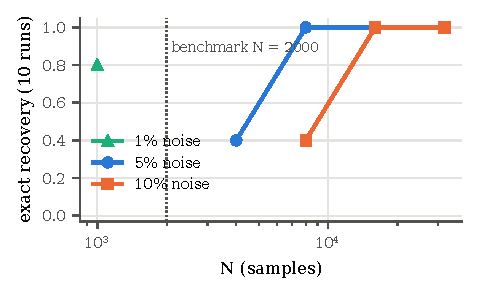
\includegraphics[width=0.5\linewidth]{figures/rf_data.pdf}
\caption{Rabinovich--Fabrikant, prospective test of the identifiability map: exact recovery by the unchanged base model on a new archive generated after the predictions were written. At $N=2000$ every method scores 0--10\%.}
\label{fig:rf}
\end{figure}

From development margins we recorded predicted identifiability probabilities for Rabinovich--Fabrikant at larger $N$ before generating new data (\cref{fig:rf}). The prediction held, conservatively: 10/10 exact at $N=8000$ with 5\% noise and at $N=16{,}000$ with 10\% noise. This shows that more data suffices for this system. It does not prove that no method could succeed at $N=2000$.


\section{Additional ablation analysis}
\label{app:ablation-detail}

The full leave-one-out rates and run-level tests are in \cref{tab:ablation}. Relative to the full method, weak-form and trajectory-segment fallbacks lose 74/2 and 87/2 paired runs. The fixed-state comparison gives 15/5 ($p=0.04$ under the pooled run-level test); this is not a system-level significance claim. In the cumulative ladder, adding proposals raises recovery by 8.7 points on sealed, from 0 to 25/40 on the hard set, and by 3.5 points on \texttt{dysts}. These conditional ablations do not isolate the effect of joint fitting independently of the candidate supports it receives.

\paragraph{Self-calibration.} On the ladder, where coloured runs still use the white-noise likelihood, proposals with the fixed high-frequency $\sigma$ and $\varphi=1$ overfit every coloured run: the exact rate falls from 0.64 to 0.00 (0/57), and self-calibration restores it (56/0). In the full method these runs go to the AR(1) model, which has its own calibration, so the corresponding row of \cref{tab:ablation} shows no change. On white noise the $\sigma/\varphi$ calibration has no measurable effect, and the self-calibrated $\sigma$ is as good as the true one, since an oracle noise level changes only one sealed and one \texttt{dysts} run.

\paragraph{Other components.} The complexity prior is small but consistent: it never loses (10/0 pooled, $p=0.002$), and its gains are spread over all four sets. The AR(1) switch helps on coloured noise (0.674 $\to$ 0.730, 9/4), though not significantly at $n=89$; on all 800 coloured runs the test pass found 23/1. With proposals in place, these sets give no evidence for multiple starts, automatic sub-steps or Huber loss. A single weak start changes nothing on white noise and is slightly \emph{better} on coloured noise (6/2 against the full model), while the design reasons for automatic sub-steps and Huber loss, stiff systems at low noise and $t_3$ noise, are not covered by these sets.

\paragraph{Huber loss under AR(1) noise.} With the Gaussian loss, the method scores 0.831 instead of 0.730 on the coloured subsample (9/0 for Gaussian, $p=0.004$). The oracle noise variant reaches a similar 0.820 (8/0), which suggests that much of the remaining coloured gap comes from noise calibration. A plausible mechanism is that Huber with $c=2$ on whitened residuals down-weights exactly the large innovations that the AR(1) likelihood needs. This was found on a test archive, so it could not be used directly, but it led to the separately confirmed change of \cref{sec:noise}.

\paragraph{Coefficients.} The median relative coefficient error over jointly exact runs barely moves under any ablation: 0.24\% on sealed and 0.60\% on the hard 40 for the full model, with variants spanning 0.22--0.83\%. Without joint states the error roughly doubles (0.58\% on sealed).

\section{Paired comparisons and timing details}
\subsection{DEDi comparison statistics}\label{app:paired}
For the 80-run comparison, the primary validation-selection comparison gives 13/2 paired wins/losses ($p=0.007$); BIC gives 7/2 ($p=0.18$). The latter meets the prospective 10-point noninferiority margin but its interval includes zero. Devices were not randomised: restricting to the 73 GPU runs gives 62 versus 54 exact and 10/2 paired wins/losses ($p=0.039$). The coloured-noise comparison alone gives 5/0 ($p=0.06$), too small to establish a general advantage.

On the 64 new-system runs, paired validation and BIC comparisons give 19/2 ($p=0.0002$) and 15/3 ($p=0.008$). The run-level Newcombe intervals for DEDi minus PJSS are $[-0.384,-0.137]$ and $[-0.306,-0.064]$; \cref{sec:h2h} reports the post-hoc system-resampled intervals. At 1--5\% noise, even the DEDi oracle recovers only 21/32, so much of the gap occurs before its final selection rule. The low-noise gap was not investigated further. \Cref{tab:h2h,tab:h2h-dysts} retain all paired results.

\subsection{Timing interpretation}\label{app:timing-detail}
On the loaded GB10 machine, PJSS takes 14--15\,s per run on one CPU core; DEDi's median full-grid time on the GPU subset is 4{,}806\,s, with a median paired ratio of 343. The GPU is shared by ten DEDi processes, and seven additional head-to-head runs use the CPU. \Cref{tab:fast} reports pooled medians, which differ from the GPU-only median.

For the three timing cases, aggregate single-thread CPU task times for DEDi are 4{,}374, 4{,}591 and 34{,}006\,s (ratios 812, 901 and 7{,}213 to PJSS); single-process GPU elapsed times are 501, 526 and 4{,}462\,s (ratios 93, 103 and 946). Each CPU total sums elapsed times of 35 pairs distributed across three simultaneous workers (12/12/11 pairs per run), rather than one serial process. The CPU ratios therefore compare aggregate task time to PJSS time, not observed serial wall time. The slowest case is Rabinovich--Fabrikant; the others are Sprott~A. One DEDi setting costs 22--29\,s on the idle GPU, and five settings cost 129--144\,s. These budgets recover 26/64 and 36/64 new-system runs, respectively. PJSS screens about 260{,}000 subsets, split between its profiled proposals and trajectory-segment starts, and performs about 21 joint fits. DEDi's repeated elimination fits across its grid dominate its cost. Scaling measurements appear in \cref{tab:anatomy}.

\section{Additional scope qualifications}
\label{app:limitations-detail}

\paragraph{Noise and identifiability.} On fresh AR(1) data recovery is 0.805, with Lorenz and Chen at 0.66--0.74. Combined heavy-tailed and correlated noise is untested. Model or discretisation error can trigger the AR(1) switch on white noise, contributing to the coarse-sampling regression. The weakest \texttt{dysts} systems contain terms contributing 0.6--1.7\% of the derivative or acting on fast time scales. The degree prior and AR(1) penalty exponent are development-selected heuristics; benchmarks with true degree above three were not evaluated.

\paragraph{Evaluation scope.} The white, coloured, $t_3$, coarse and held-out archives were reused during development. The external \texttt{dysts}, hard-120, fresh coloured and fresh noise-free archives provide the separate confirmations described in the protocol. Pooled run-level tests do not establish performance on independent new systems. DEDi's GPU runs are not bit-reproducible between repeats; its first comparison has only 16 runs per condition. The $D>3$ sparse-regression baselines are minimal reimplementations. Partial-observation evaluation allows affine latent gauges, rejects valid non-affine gauges, and costs minutes rather than seconds per run.

\paragraph{Model inadequacy.} On the measured double pendulum, PJSS breaks kinematic identities preserved by equation-wise baselines. Contamination between equations through the joint fit is a proposed explanation, not an experimentally isolated cause. The ambiguity flag and confidence calibration were validated on in-library systems and cannot certify library adequacy.


\section{Audit of validation and reproducibility}
\label{app:baseline-audit}
The historical weak-feature baseline tables use PySINDy's randomly sampled weak domains. The benchmark runner seeded its optimisers after domain construction, so the domains were not reproducibly tied to each run index. The corrected runner seeds domain construction first and records the seed policy. Historical records remain unchanged and are not represented as results of the corrected code. \path{benchmarks/audit_weak_seed.py} checks corrected runs in opposite orders after perturbing worker RNG state and compares a small, outcome-independent subset with the historical records. This is a reproducibility diagnostic, not a replacement benchmark.

The targeted check uses eight weak-STLSQ, four weak-SR3 and two weak-E-SINDy runs, selected across noise/length cells before fitting. All 14 corrected records repeat identically after reversing execution order and perturbing the preceding RNG state. Relative to the historical records, CV-selected supports change in 12/14 cases and AICc-selected supports in 13/14; pooled exact recovery remains 2/14 for CV and changes from 0/14 to 1/14 for AICc. The sample is too small to establish the full-archive effect. It verifies repeatability in the current environment, not historical-result equivalence; software-environment differences may also contribute to the historical discrepancies. The saved diagnostic is \path{results_submission_audit/weak_seed_verified.json}.

CV splits consecutive regression-row indices after features have been computed on the full record. For weak features these indices do not define disjoint time intervals; domains can overlap across folds. For SFD features the rows are time-ordered but smoothing crosses fold boundaries. These scores compare regression predictions under shared preprocessing, not forecasting on unseen time blocks. The oracle references and external support-recovery comparisons remain descriptive evidence, but the CV results alone do not establish the performance of a strictly time-separated selection rule.

\subsection{System-bootstrap intervals}
\label{app:bootstrap}
The original system-bootstrap seeds and implementation were not preserved. We therefore recomputed the reported system intervals from the stored records with \path{benchmarks/audit_system_intervals.py}: 100{,}000 replicates, NumPy default RNG seed 20261102, sorted system labels, and percentile endpoints at 2.5\% and 97.5\%. Each replicate samples the original number of systems with replacement, retaining every run in each sampled system, and computes the pooled run rate or paired difference. This post-hoc audit reproduces the qualitative conclusions but replaces undocumented historical endpoints; it is not a new algorithm evaluation. The run-level Newcombe intervals are unchanged.

\subsection{Availability and evidence preservation}
\label{app:data-audit}
The submission audit checks all 47 manifest entries: 43 originals are present and match SHA-256, including ten documented relocations; four are absent. The missing files are \path{po_test.npz}, \path{dev_clean.npz}, \path{sealed_clean.npz} and \path{dysts_precdev.npz}, affecting partial-observation and noise-free/precision studies. Replaying their documented generators in the current environment produced different hashes. These alternatives are retained separately and do not replace the original experimental inputs. For the precision development archive, even the regenerated sidecar differs numerically; the cause has not been isolated.

Auditing saved coefficients reproduces their stored metrics across the full \texttt{dysts} archives and selected official-baseline models. All 5{,}250 saved DEDi fits have complete grids and matching coefficient-derived metrics. The external PJSS comparison and profiling variants retain metrics but not fitted coefficients, so their coverage and aggregates can be checked but their supports cannot be independently rescored from those records. Oracle baseline paths likewise lack complete coefficient histories. The JSON audits record input hashes and these limits. These checks support reporting consistency; they are not independent reruns of the algorithms.


\end{document}
